% Dokumentinformationen
%Vorlage erstellt von Luca Mazzoleni aufbaudend auf der Vorlage von Stefan Reinli

% !TeX program = pdflatex
% !TeX encoding = utf8
% !TeX spellcheck = en_En
% !BIB program = bibtex

\documentclass[
11pt,
final,
twoside,
a4paper]{article}
%%%%
%pachages to generate images


% Document information
\newcommand*{\Title}            {Design of a Fully Integrated Buck-Boost Converter ASIC}
\newcommand*{\TitleInfo}        {A small buck-boost converter ASIC with integrated switches on a commercial 0.35 um process node for use in a charging case for hearing devices}
\newcommand*{\AuthorOne}		{Matthias Meyer}
\newcommand*{\AuthorTwo}		{Patrick Jansky}
\newcommand*{\Author}			{\AuthorOne, \AuthorTwo}
\newcommand*{\Prof}				{Prof. Dr. Paul Zbinden}
\newcommand*{\Exam}             {Lars Kamm}
\newcommand*{\Studiengang}		{Electrical Engineering (ElE) }
\newcommand*{\Place}            {Rapperswil}
\newcommand*{\LogoOST}          {
\includegraphics[height = 0.9cm]{header/Ost_Logo}}
\newcommand*{\LogoCompany}      {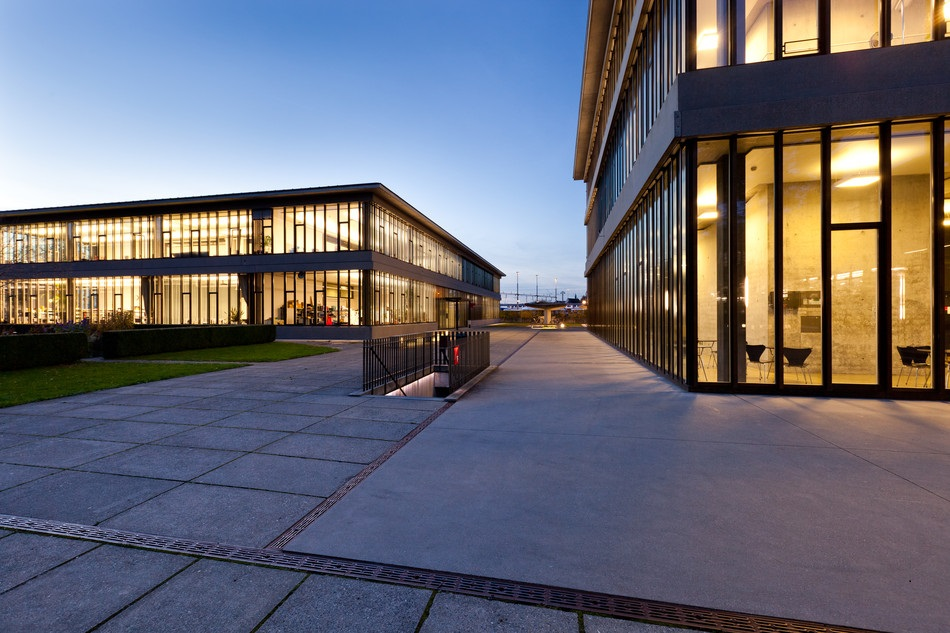
\includegraphics[height = 0.9cm]{header/logo}}
%\newcommand*{\LogoInstitute}    {
\includegraphics[height = 1cm]{header/ICOM_Logo_2.png}}
\newcommand*{\Print}            {true} % true for black links (print version), false for color links (pdf version)

% Header
%Change the folliwing line in tikz
\usepackage[subpreambles=true]{standalone}
%\usepackage[mode=build]{standalone}
%package to import images

%\usepackage{import}


%Set language to english PJ
%\usepackage[ngerman]{babel} % Silbentrennung und Rechtschreibung Deutsch
\usepackage[english]{babel} % Silbentrennung und Rechtschreibung Deutsch
\usepackage[{left=1.5cm,right=1.5cm,top=0cm,bottom=0cm}]{geometry} % Seitenränder Titelblatt


%%%%%%%%%%%%%%%%%%%%%%%
%% Packages
%%%%%%%%%%%%%%%%%%%%%%%
\usepackage[page,header]{appendix}

\usepackage{acronym} 		   % Für Abkürzungsverzeichnis
\usepackage{adjustbox} 		   % adjustbox, minipage..
\usepackage{amsmath}   		   % Allgemeine Matheumgebungen
\usepackage{amssymb}  		   % Fonts: msam,msbm, eufm & Mathesymbole, Mengen (lädt automatisch amsfonts)
\usepackage{array} 			   % Extending the array and tabular environment -> m,b,p,..
\usepackage{caption}  		   % Verändern der Schriftart von Bildunterschriften
\usepackage{changepage}
\usepackage{csquotes}
\usepackage{epstopdf}
\usepackage{expl3}
\usepackage{float}
\usepackage{framed, color}
\usepackage{fancyhdr}			%Für Kopf & Fusszeile
\usepackage{graphbox}
\usepackage{graphicx}
\usepackage{titletoc}			% Editieren des TOCs muss vor hyperref geladen werden
\usepackage{tocloft}			% Editieren des TOCs muss vor hyperref geladen werden
\usepackage{hyperref}
\usepackage{hyphenat}			%Wortumbruch
\hyphenation{he-lio-trope opos-sum}
\usepackage[table]{xcolor}
\usepackage{listings}           % Erlaubt es Programmcode in der gewünschten Sprache zu hinterlegen (C++, Matlab,..)
\usepackage{longtable}
\usepackage{lastpage}			%Lastpage ref for Footer
\usepackage{marginnote} 		% Für Seitenkommentare \marginnote
\usepackage{mathtools}          % Vor mathabx laden!
\usepackage{mathabx} 			% Package mit vielen weiteren Mathe Symbolen
\usepackage{mparhack}  			% Improved marginpar placement
\usepackage{multicol} 			% In­ter­mix sin­gle and mul­ti­ple columns
\usepackage{multirow} 			% Create tabular cells spanning multiple rows
\usepackage{paralist}
\usepackage{pdfpages} 
\usepackage{pxfonts} 			% Mathsymbols
\usepackage[section]{placeins}  % Float-Barrier for Section
\usepackage{rotating} 			% Rotation tools, including rotated fullpage floats
\usepackage[onehalfspacing]{setspace}

\usepackage{subcaption}
\usepackage{tabularx}
\usepackage{textcomp} 			% Wird für Copyright-Symbol,Währungen, Musikalische-Symbole benötigt
\usepackage[colorinlistoftodos,prependcaption,textsize=tiny]{todonotes}
\usepackage[most]{tcolorbox}
\usepackage{trfsigns}
\usepackage{varwidth}
\usepackage{wrapfig}
%Include package for pdf with plack background
\usepackage[framemethod=TikZ]{mdframed}
\usepackage{environ}
\usepackage{varwidth}

\newlength{\MyMdframedWidthTweak}%
\NewEnviron{MyMdframed}[1][]{%
	\setlength{\MyMdframedWidthTweak}{\dimexpr%
		+\mdflength{innerleftmargin}
		+\mdflength{innerrightmargin}
		+\mdflength{leftmargin}
		+\mdflength{rightmargin}
	}%
	\savebox0{%
		\begin{varwidth}{\dimexpr\linewidth-\MyMdframedWidthTweak\relax}%
			\BODY
		\end{varwidth}%
	}%
	\begin{mdframed}[
		roundcorner=5pt,
		userdefinedwidth=\dimexpr\wd0+\MyMdframedWidthTweak\relax, 
		#1]
		\usebox0
	\end{mdframed}
}
%Include package to colorize code
\usepackage{minted}
\usemintedstyle{borland}
\usepackage{scrhack}        	% Fixes koma-script incompatibilities
\usepackage[T1]{fontenc}	% ä,ü...
\usepackage[utf8]{inputenc} % utf-8 Unterstützung
\definecolor{black}{cmyk}{0,0,0,1}             
\definecolor{white}{cmyk}{0,0,0,0}
\definecolor{darkgrey}{cmyk}{0,0,0,0.97}      %background in Visual Studio
\definecolor{lightgrey}{cmyk}{0,0,0,0.67}
\definecolor{green}{cmyk}{0.6,0,0.84,0}       %comments in Visual Studio
\definecolor{blue}{cmyk}{0.65,0.33,0,0.05}       %keywords in Visual Studio
\definecolor{rose}{cmyk}{0,0.26,0.38,0}       %strings in Visual Studio
\definecolor{lavender}{cmyk}{0,0.42,0,0.1}   %if/else,switch/case etc. in Visual Studio
\definecolor{lightblue}{cmyk}{0.35,0,0,0}     %local variables in Visual Studio
\definecolor{aqua}{cmyk}{0.65,0,0.23,0}       %class types in Visual Studio
\definecolor{lightgreen}{cmyk}{0.12,0,0.33,0.05} %enumerations and methods in Visual Studio
\usemintedstyle[bash, bat]{boreland}
\usemintedstyle[vhdl]{manni}
\setminted[vhdl]{frame=lines,framesep=2mm,baselinestretch=1.2,linenos,breaklines}
\usemintedstyle[matlab]{manni}
\setminted[matlab]{frame=lines,framesep=2mm,baselinestretch=1.2,linenos,breaklines}
\usemintedstyle{fruity}
\setminted[bat]{frame=lines,framesep=2mm,baselinestretch=1.2,bgcolor=lightgrey,linenos,breaklines}
%Make it possible to go to new page
\newenvironment{longlisting}{\captionsetup{type=listing}}{}


%%%%%%%%%%%%%%%%%%%%%%%
%% PDF Meta Data
%%%%%%%%%%%%%%%%%%%%%%%

\hypersetup{pdftex,
pdfauthor={\Author},
pdftitle={\Title},
pdfsubject={\TitleInfo},
%pdfkeywords={Some Keywords},
pdfproducer={Latex with hyperref}
%pdfcreator={pdflatex}
}

%%%%%%%%%%%%%%%%%%%%%%%
%% Setup Tikz
%%%%%%%%%%%%%%%%%%%%%%%

\usepackage{tikz}
\usetikzlibrary{arrows.meta}
\usetikzlibrary{hobby}

%\usepackage{struktex}
%\usepackage{schemabloc}
%\usepackage[normalem]{ulem}
%\usetikzlibrary{circuits}
%\usetikzlibrary{arrows}
%\usetikzlibrary{circuits.ee.IEC}
%\usetikzlibrary{patterns}
%\usetikzlibrary{positioning}
%\usetikzlibrary{shapes,arrows}
%
%\usepackage{pgfplots}
%\usepackage{pgfplotstable}
%\pgfplotsset{compat=newest}
%
%\tikzstyle{block} = [draw, rectangle, minimum height=3em, minimum width=4em]
%\tikzstyle{input} = [coordinate]
%\tikzstyle{output} = [coordinate]
%\tikzstyle{pinstyle} = [pin edge={to-,thin,black}]
%\tikzstyle{sum} = [draw, circle, node distance=1em, minimum height=1.5em]
%\tikzset{>=latex}
%\tikzset{%
%	block/.style    = {draw, thick, rectangle, minimum height = 3em,
%		minimum width = 3em},
%	sum/.style      = {draw, circle, node distance = 1.5cm}, % Adder
%	input/.style    = {coordinate}, % Input
%	output/.style   = {coordinate} % Output
%}
%\newcommand\Umbruch[2][3cm]{\begin{varwidth}{#1}\centering#2\end{varwidth}}

%%%%%%%%%%%%%%%%%%%%%%%
% Caption Setup
%%%%%%%%%%%%%%%%%%%%%%%
\captionsetup[figure]{labelfont={it,bf},textfont={it}}
\captionsetup[table]{labelfont={it,bf},textfont={it},singlelinecheck=off,justification=centering}
\captionsetup[lstlisting]{labelfont={it,bf},textfont={it}}
\captionsetup[subfigure]{labelfont=bf,textfont=normalfont,singlelinecheck=off,justification=centering}

\newenvironment{nscenter}
{\parskip=-5pt\par\nopagebreak\centering}
{\parskip=-15pt\par\noindent\ignorespacesafterend}


\setlength{\cftfignumwidth}{2cm}	% Width of equation number in List of Figure
\setlength{\cfttabnumwidth}{2cm}	% Width of equation number in List of Table

%List of Equations
\newcommand{\listequationsname}{Gleichungen}
\newlistof{myequations}{equ}{\listequationsname}
\newcommand{\myequations}[1]{% 
    \addcontentsline{equ}{myequations}{\protect\numberline{\theequation}#1}\par}
\setlength{\cftmyequationsnumwidth}{2cm}% Width of equation number in List of Equations


%%%%%%%%%%%%%%%%%%%%%%%%
%% Header and Footer %%
%%%%%%%%%%%%%%%%%%%%%%%%
\pagestyle{fancy} %eigener Seitenstil
\renewcommand{\sectionmark}[1]{\markright{#1}} %entfernt nummer vor section
\renewcommand{\subsectionmark}[1]{}
%twopage
%\ifthenelse{\isodd{\value{page}}}{\leftmark}{\rightmark}
% or with
%\fancyhead[OR]{} % "O" for "odd"
%\fancyhead[ER]{} % "E" for "even"

\fancypagestyle{plain}{
    \fancyhf{} %alle Kopf- und Fußzeilenfelder bereinigen
    
    \fancyhead[OR]{\LogoOST}
%    \fancyhead[ER]{\LogoInstitute}
    \fancyhead[C]{\textsl{\rightmark}} %zentrierte Kopfzeile
%    \fancyhead[OL]{\LogoInstitute}
    \fancyhead[EL]{\LogoOST}
    \renewcommand{\headrulewidth}{0.4pt} %obere Trennlinie
    
    %\fancyfoot[OR]{Seite \thepage\ / \pageref{LastPage}}
    \fancyfoot[OR]{Page \thepage\ / \pageref{LastPage}}
    \fancyfoot[ER]{\small{\Author}}
    %\fancyfoot[C]{\small{\Title}}
    \fancyfoot[EL]{Page \thepage\ / \pageref{LastPage}}
    \fancyfoot[OL]{\small{\Author}}
    \renewcommand{\footrulewidth}{0.4pt} %untere Trennlinie
}

\fancypagestyle{appendix}{
    \fancyhf{} %alle Kopf- und Fußzeilenfelder bereinigen
    \fancyhead[R]{} %Kopfzeile links
    \fancyhead[C]{} %zentrierte Kopfzeile
    \fancyhead[L]{} %Kopfzeile rechts
    \renewcommand{\headrulewidth}{0pt} %obere Trennlinie
    
    \fancyfoot[OR]{Page \thepage\ / \pageref{LastPage}}
    \fancyfoot[ER]{\today}
    \fancyfoot[C]{}
    \fancyfoot[EL]{Page \thepage\ / \pageref{LastPage}}
    \fancyfoot[OL]{\today}
    \renewcommand{\footrulewidth}{0.4pt} %untere Trennlinie
}


\pagestyle{plain} %Pagesytle


%%%%%%%%%%%%%%%%%%%%%
%% Load HSR Color  %%
%%%%%%%%%%%%%%%%%%%%%

\usepackage{header/HSRColors}

%%%%%%%%%%
% Colors %
%%%%%%%%%%
\definecolor{black}{rgb}{0,0,0}
\definecolor{red}{rgb}{1,0,0}
\definecolor{white}{rgb}{1,1,1}
\definecolor{grey}{rgb}{0.8,0.8,0.8}
\definecolor{green}{rgb}{0,.8,0.05}
\definecolor{brown}{rgb}{0.603,0,0}
\definecolor{mymauve}{rgb}{0.58,0,0.82}
\definecolor{mygreen}{RGB}{28,172,0}
\definecolor{mygray}{rgb}{0.5,0.5,0.5}
\definecolor{mymauve}{rgb}{0.58,0,0.82}
\definecolor{mylilas}{RGB}{170,55,241}

\definecolor{gray80}{gray}{0.8}
\definecolor{gray60}{gray}{0.6}
\definecolor{gray40}{gray}{0.4}
\definecolor{gray20}{gray}{0.2}

%%%%%%%%%%%%%%%%%%%%%
%% Title %%
%%%%%%%%%%%%%%%%%%%%%



%Title Spacing-----------------------------------------
\usepackage{titlesec}
%\titlespacing{name=\section}{-\marginparwidth}{0pt}{0.2em}
%\titlespacing{name=\subsection}{-\marginparwidth+10pt}{0pt}{0.2em}
%\titlespacing{name=\subsubsection}{-\marginparwidth+14pt}{0.2em}{0.2em}
%\titlespacing{name=\paragraph}{-\marginparwidth+18pt}{0.2em}{0.2em}

\titlespacing{name=\section}{1pt}{0pt}{0.2em}
\titlespacing{name=\subsection}{1pt}{0pt}{0.2em}
\titlespacing{name=\subsubsection}{1pt}{0.2em}{0.2em}
\titlespacing{name=\paragraph}{1pt}{0.2em}{0.2em}

%%%%%%%%%%%%%%%%%%
%% Bibliography %%
%%%%%%%%%%%%%%%%%%
%\usepackage[fixlanguage]{babelbib}
%\selectbiblanguage{german}
\usepackage[backend=bibtex,style=ieee, defernumbers=true]{biblatex} %Do not use biber with TexWorks
\addbibresource{Literatur}


% Abbildungen im Quellenverzeichnis nach Alphabet ordnen, Rest nummerieren
%\DeclareFieldFormat{labelnumber}{\ifkeyword{abb}{\mknumalph{#1}}{#1}}


%%%%%%%%%%%%%%%%%%%%%%%%%%%%%%%%%%%
%% Itemize and Enumerate spacing %%
%%%%%%%%%%%%%%%%%%%%%%%%%%%%%%%%%%%
% \topsep: space between first item and preceding paragraph
% \partopsep: extra space added to \topsep when environment starts a new paragraph
% \itemsep: space between successive items. 
\usepackage{enumitem} % Controls Layout of itemize, enumerate, description
\setlist[itemize]{topsep=0pt,itemsep=-1ex,partopsep=1ex,parsep=1ex,after=\vskip0.1\baselineskip}
\setlist[enumerate]{topsep=0pt,itemsep=-1ex,partopsep=1ex,parsep=1ex,after=\vskip0.1\baselineskip}

%%%%%%%%%%%
%% Index %%
%%%%%%%%%%%
\usepackage{imakeidx}
\makeindex[intoc,columnseprule]
\indexsetup{firstpagestyle=plain}    % Show header/footer on index page

%-------------------------------------------------
% Marginalien/Seitenränder
%-------------------------------------------------
%\marginpar{Eine Randnotiz}
\newcommand{\marg}[1]{\marginpar{\raggedright \textbf{#1} }}	

%%%%%%%%%%%%%%%%%%%%%%%
%% Aligned footnotes %%
%%%%%%%%%%%%%%%%%%%%%%%
\usepackage[hang]{footmisc}
\setlength{\footnotemargin}{1em}

%%%%%%%%%%%%%
%% Tabular %%
%%%%%%%%%%%%%
\newcolumntype{L}[1]{>{\raggedright\arraybackslash}p{#1}} % Tabelleninhalt linksausgerichtet
\newcolumntype{R}[1]{>{\raggedleft\arraybackslash}p{#1}} % Tabelleninhalt rechtsausgerichtet
\newcolumntype{C}[1]{>{\centering\arraybackslash}p{#1}} %  Tabelleninhalt zentriert


%%%%%%%%%%%%%%%%%%%%%%
%% Generelle Makros %%
%%%%%%%%%%%%%%%%%%%%%%

% If \Print=true, then make all links black for nicer print
\providecommand*{\True}{true}
\ifx \Print \True
\hypersetup{hidelinks, colorlinks, linkcolor = black, citecolor = black, filecolor = black, urlcolor = black}
\fi

\parindent0pt % Zeileneinzug verhindern

%Matlab font
\newcommand{\matlab}[1]{\footnotesize{(Matlab: \texttt{#1})}\normalsize{}}

% Makro für Tabellenbilder gleich unterhalb der Linie
\newcommand\tabbild[2][]{%
	\raisebox{0pt}[\dimexpr\totalheight+\dp\strutbox\relax][\dp\strutbox]{%
		\includegraphics[#1]{#2}%
	}%
}

% Makro für Vorteile und Nachteil mit Plus und Minus
\newcommand\pro{\item[$+$]}
\newcommand\con{\item[$-$]}


%Float-Barrier for Subsection
\makeatletter
\AtBeginDocument{%
	\expandafter\renewcommand\expandafter\subsection\expandafter{%
		\expandafter\@fb@secFB\subsection
	}%
}
\makeatother


%%%%%%%%%%%%%%%%%%%%%%%%%%%%
% Mathematical Operators %
%%%%%%%%%%%%%%%%%%%%%%%%%%%%
\DeclareMathOperator{\sinc}{sinc}
\DeclareMathOperator{\sgn}{sgn}
\DeclareMathOperator{\Real}{Re}
\DeclareMathOperator{\Imag}{Im}
\DeclareMathOperator{\euler}{e}
\DeclareMathOperator{\cov}{cov}
\DeclareMathOperator{\PolyGrad}{PolyGrad}
\DeclareMathOperator{\gradient}{grad}
\DeclareMathOperator{\rotation}{rot}
\DeclareMathOperator{\divergenz}{div}
\DeclareMathOperator{\imag}{j}

%Grösse Integral anpassen
\def\Int{\mbox{\Large$\displaystyle\int$\normalsize}}
\def\Int{\mbox{\Large$\displaystyle\iint$\normalsize}}
\def\OInt{\mbox{\Large$\displaystyle\oint$\normalsize}}

%Makro für 'd' von Integral- und Differentialgleichungen 
\newcommand*{\diff}{\mathop{}\!\mathrm{d}}

%%%%%%%%%%%%%%%%%%%%%%%%%%%
% Fouriertransform %
%%%%%%%%%%%%%%%%%%%%%%%%%%%

\unitlength1cm
\newcommand{\FT}
{
	\begin{picture}(1,0.5)
	\put(0.2,0.1){\circle{0.14}}\put(0.27,0.1){\line(1,0){0.5}}\put(0.77,0.1){\circle*{0.14}}
	\end{picture}
}


\newcommand{\IFT}
{
	\begin{picture}(1,0.5)
	\put(0.2,0.1){\circle*{0.14}}\put(0.27,0.1){\line(1,0){0.45}}\put(0.77,0.1){\circle{0.14}}
	\end{picture}
}


%%%%%%%%%%%%%%%%%%%%%%%%%%%
% Tikzimage %
%%%%%%%%%%%%%%%%%%%%%%%%%%%
\usepackage{graphics}
\usepackage{siunitx}
\usepackage{tikz}
\usepackage{pgfplots}
\pgfplotsset{compat=newest} 
\usepackage[%
  europeanvoltages,
  europeancurrents,
  europeanresistors,
  americaninductors,
  smartlabels]{circuitikz}

\usetikzlibrary{calc}
\ctikzset{bipoles/thickness=1}
\ctikzset{bipoles/length=0.8cm}

\ctikzset{resistors/scale=1.2, % smaller R
 capacitors/scale=1, % even smaller C
 diodes/scale=1, % small diodes
 inductors/scale=1.4, % small inductors
 transistors/scale=1.5} % bigger BJTs
\tikzstyle{every node}=[font=\small]
%\tikzstyle{every path}=[line width=0.8pt,line cap=round,line join=round]


%%%%%%%%%%%%%%%%%%%%%%%%%%%%%%%%%%%%%This is used for the table of units%%%%%%%%%%%%%%%%%%%%%%%%%%%%%%%
%\usepackage{amssymb}
\usepackage{nomencl}
%\usepackage{siunitx}
%\usepackage{hyperref}
\makenomenclature
\hypersetup{
	colorlinks=true,
	urlcolor=blue,
}
%% This will add the subgroups
%----------------------------------------------
\usepackage{etoolbox}
\renewcommand\nomgroup[1]{%
	\item[\bfseries
	\ifstrequal{#1}{A}{Physics Constants}{%
		\ifstrequal{#1}{B}{Number Sets}{%
			\ifstrequal{#1}{C}{Other Symbols}{}}}%
	]}
%----------------------------------------------

%% This will add the units
%----------------------------------------------
\newcommand{\nomunit}[1]{%
	\renewcommand{\nomentryend}{\hspace*{\fill}#1}}
%%%%%%%%%%%%%%%%%%%%%%%%%%%%%%%%%%%%%This is used for the table of units%%%%%%%%%%%%%%%%%%%%%%%%%%%%%%%

%%%%%%%%%%%%%%%%
% Code Layout %
%https://en.wikibooks.org/wiki/LaTeX/Source_Code_Listings
%%%%%%%%%%%%%%%

%\definecolor{mygreen}{rgb}{0,0.6,0}
%\definecolor{mygray}{rgb}{0.5,0.5,0.5}
%\definecolor{mymauve}{rgb}{0.58,0,0.82}

\lstset{ %
    firstnumber=1,
    backgroundcolor=\color{white},   % choose the background color; you must add        \usepackage{color} or \usepackage{xcolor}
    basicstyle=\footnotesize\ttfamily, % the size of the fonts that are used for the code
    breakatwhitespace=false,         % sets if automatic breaks should only happen at whitespace
    breaklines=true,                 % sets automatic line breaking
    captionpos=b,                    % sets the caption-position to bottom
    commentstyle=\color{mygreen},    % comment style
    deletekeywords={...},            % if you want to delete keywords from the given language
    otherkeywords={...},             % if you want to add more keywords to the set
    escapeinside={\%*}{*\%},          % if you want to add LaTeX within your code
    extendedchars=true,              % lets you use non-ASCII characters; for 8-bits encodings only, does not work with UTF-8
    frame=single,	                 % adds a frame around the code
    keepspaces=true,                 % keeps spaces in text, useful for keeping indentation of code (possibly needs columns=flexible)
    keywordstyle=\color{blue},       % keyword style
    language=C++,                    % the language of the code   
    numbers=left,                    % where to put the line-numbers; possible values are (none, left, right)
    numbersep=5pt,                   % how far the line-numbers are from the code
    numberstyle=\tiny\color{mygray}, % the style that is used for the line-numbers
    rulecolor=\color{black},         % if not set, the frame-color may be changed on line-breaks within not-black text (e.g. comments (green here))
    showspaces=false,                % show spaces everywhere adding particular underscores; it overrides 'showstringspaces'
    showstringspaces=false,          % underline spaces within strings only
    showtabs=false,                  % show tabs within strings adding particular underscores
    stepnumber=2,                    % the step between two line-numbers. If it's 1, each line will be numbered
    stringstyle=\color{mymauve},     % string literal style
    tabsize=2,	                     % sets default tabsize to 2 spaces
    %title=\lstname                   % show the filename of files included with         \lstinputlisting; also try caption instead of title
}

\lstdefinestyle{customc++}{
    belowcaptionskip=1\baselineskip,
    %frame=L,
    xleftmargin=\parindent,
    language=C++,
    keywordstyle=\bfseries\color{blue},
    commentstyle=\itshape\color{mygreen},
    identifierstyle=\color{black},
    stringstyle=\color{gray},
}

\lstdefinestyle{cppunit}{
    belowcaptionskip=1\baselineskip,
    %frame=L,
    xleftmargin=\parindent,
    language=C++,
    keywordstyle=\bfseries\color{blue},
    keywordstyle=[2]\bf\color{black}, %not sure why \bf works, but it does
    commentstyle=\itshape\color{mygreen},
    identifierstyle=\color{black},
    stringstyle=\color{gray},
    keywords=[2]{  %Cpp Unit Keywords
        CPPUNIT_ASSERT,
        CPPUNIT_TEST,
        CPPUNIT_TEST_EXCEPTION,
        CPPUNIT_TEST_END,
        CPPUNIT_TEST_SUITE,
        CPPUNIT_TEST_SUITE_REGISTRATION,
        CPPUNIT_TEST_SUITE_END},
}

\lstdefinestyle{cppqt}{
    belowcaptionskip=1\baselineskip,
    %frame=L,
    xleftmargin=\parindent,
    language=C++,
    keywordstyle=\bfseries\color{blue},
    keywordstyle=[2]\bfseries\color{red},
    commentstyle=\itshape\color{mygreen},
    identifierstyle=\color{black},
    stringstyle=\color{gray},
    keywords=[2]{           % qt-Keywords
		Qt,
        SIGNAL,
        SLOT,
        QApplication,
        QDialog,
        QGridLayout,
        QPushButton,
        QLabel,
        QVBoxLayout,
        QHBoxLayout,
        QWidget,
        QGroupBox,
        QFont,
        QLineEdit,
        QRadioButton,
        QPen,
        QRect,
        QPaintEvent,
        QBrush,
        QPixmap,
        QPainter,
        QString,
        QPoint,
        update()},
}

\lstdefinestyle{cdoxy}{
    belowcaptionskip=1\baselineskip,
    %frame=L,
    xleftmargin=\parindent,
    language=C++,  
    keywordstyle=\bfseries\color{blue},
    commentstyle=\itshape\color{mygreen},
    identifierstyle=\color{black},
    stringstyle=\color{gray},
    otherkeywords={           % DoxygenKeywords
        ...,
        ....,
        @mainpage,
        @file,
        @author,
        @version,
        @date,
        @bug,
        @brief,
        @extended,
        @param,
        @return,
        @warning,
        @note,
        @see},
}

\lstdefinestyle{custommatlab}{
	belowcaptionskip=1\baselineskip,
	%frame=L,
	xleftmargin=\parindent,
	language=Matlab,
	basicstyle=\footnotesize\ttfamily,
	keywordstyle=\bfseries\color{blue},
	commentstyle=\itshape\color{mygreen},
	identifierstyle=\color{black},
	stringstyle=\color{mylilas},
}

%choose customstyle in DOC with \lstinputlisting[style=custom]{path}
\lstset{style=customc++}

\setcounter{secnumdepth}{4}

%\includeonly{sections/Einleitung,sections/Einleitung1,sections/Verzeichnisse}


% tcolorbox setup
\tcbset{width=(\linewidth-1mm)/2,before=,after=\hfill,arc=0mm,
	colframe=red!50!black,colback=white,colback = red!10}

\newcommand{\hsp}{\hspace{20pt}}
\titleformat{\section}[hang]{\Huge\bfseries}{\thesection\hsp\textcolor{gray80}{|}\hsp}{0pt}{\Huge\bfseries}
\titleformat{\subsection}[hang]{\huge\bfseries}{\thesubsection\hsp\textcolor{gray60}{|}\hsp}{0pt}{\Large\bfseries}
\titleformat{\subsubsection}[hang]{\Large\bfseries}{\thesubsubsection\hsp\textcolor{gray40}{|}\hsp}{0pt}{\large\bfseries}
\titleformat{\paragraph}[hang]{\large\bfseries}{\theparagraph\hsp\textcolor{gray20}{|}\hsp}{0pt}{\large\bfseries}

% fontstyle
%\renewcommand\familydefault{\sfdefault}    % Arial
% Document=========================================
\begin{document}
    \pagenumbering{Roman}
    \thispagestyle{empty}
    \begin{titlepage}
	
	\begin{adjustwidth}{-25mm}{-45mm}
		%Seite einmitteln gemäss werten im geometry package:		
		\begin{adjustwidth}{35mm}{40mm}
			\textsf{
				%\textsf{	%sans serif schrift
				\vspace*{2cm}
				\begin{flushleft}
					\Huge \textbf{\Title}\\
					\vspace{.25cm}
					\Large \sffamily\TitleInfo \\
				\end{flushleft}
			}
		\end{adjustwidth}
		
		\begin{figure}[H]
	        \centering
        	%\includegraphics[width=0.8\textwidth]{images/Titelblatt_V2.png}
	        
        \end{figure}
		
		\begin{adjustwidth}{35mm}{40mm}	
			\vfill
			\large
			\textsf{\textbf{Autors}}\\
			\textsf{\Author} \\
			\textsf{\textbf{Professor}}\\
			\textsf{\Prof}\\
			\textsf{\textbf{Experts}}\\
			\textsf{\Exam}\\
			\textsf{\textbf{Study}}\\
			\textsf{\Studiengang}\\
			\textsf{\textbf{Subject Area}}\\
			\textsf{Microelectronics}\\
			\hfill\hbox{}\\
			\textsf{OST RJ Ostschweizer Fachhochschule Rapperswil}\\
			\hfill\hbox{}\\
			\textsf{\today}
            \vspace{3cm}
		\end{adjustwidth}		
	\end{adjustwidth}
\end{titlepage}

    \clearpage \pagebreak
    \thispagestyle{empty}
    %\listoftodos
    \cleardoublepage \pagebreak
    \pagenumbering{arabic}
    \setcounter{page}{1}
    \thispagestyle{empty}

\newgeometry{left=2cm,right=4cm,top=1cm,bottom=1cm,headsep=1.5cm, marginparwidth=30mm,marginparsep=3mm,includeheadfoot}
\savegeometry{margin}
	\thispagestyle{empty}
	\section*{\huge Abstract}
\label{chap:abstract}
This document focuses on the pre-layout phase of a project, which was divided into pre-layout and post-layout stages. The project was initiated by Sonova AG, with the objective of designing a compact 200 mA DC/DC converter for potential integration into the charging case of their hearing devices. This first part of the documentation provides a comprehensive overview of the key steps undertaken during the pre-layout phase, including DC/DC topology selection, circuit architecture/design, and chip interface considerations. By examining these crucial aspects, this documentation offers valuable insights into the initial phase of the project, providing a solid foundation for the subsequent layout and manufacturing, and testing stages.
\clearpage
	\section*{\huge Acknowledgements}
\label{chap:danksagung}
We would like to express our sincere gratitude to our advisor, Lars Kamm, for his guidance and support throughout this project. His expertise and insights were invaluable in helping us navigate the complexities of \ac{ASIC} design. We would also like to thank the team at OST Rapperswil for providing us with the resources and environment necessary to carry out this project.
%We would like to express our deepest gratitude and appreciation to all those who have contributed to the first part of this project. Without their support, guidance, and encouragement, this work would not have been possible.\\\\
%First and foremost, We are immensely grateful to our supervisor, Lars Kamm, for his unwavering support and invaluable guidance throughout this first part of the project. His expertise, patience, and dedication has been instrumental in shaping and refining this project. We are truly fortunate to have had such a knowledgeable and inspiring supervisor.\\\\
%We extend our heartfelt appreciation to the faculty members of IMES (Institut für Mikroelektronik und Embedded Systems) at OST, whose profound insights and constructive feedback have greatly enhanced the quality of this project. Their commitment to analog and digital design has been a constant source of motivation for us. Moreover, we would like to express our deep appreciation to the department's support in providing us with a physical workspace in middle of the team.\\\\
%In conclusion, we are deeply grateful to all those who have contributed to this work in various ways. Their collective efforts have played a significant role in shaping this project and making it possible.\\\\


%We are immensely grateful to our supervisor, Lars Kamm, for his invaluable feedback and guidance throughout this project. His profound expertise in the field of \ac{ASIC} design has been crucial in directing us and shaping the project, enabling us to present our results here today. \\
%We would like to express our gratitude to the faculty members of IMES (Institut für Mikroelektronik und Embedded Systems) at OST for lending us a helping hand in times of need. A special thanks goes out to Lukas Leuenberger, Simon Walker and Roman Willi for their endless hours helping us get acquainted with the tools we required and answering our many questions regarding analog circuit design. \\
%Finally, we are profoundly grateful to Prof. Dr. Paul Zbinden for giving us this rare opportunity, to design a fully custom integrated circuit as part of our masters program.\\
%Thank you all.

%\textcolor{red}{TBD}

\clearpage

\newgeometry{left=2cm,right=2cm,top=1cm,bottom=1cm,headsep=1.5cm, marginparwidth=1mm,marginparsep=3mm,includeheadfoot} %Seitenränder Dokument ohne Titelblatt und Abstract



\savegeometry{no-margin}
	\begin{spacing}{1}
		\startcontents[sections]
		\printcontents[sections]{l}{1}{\setcounter{tocdepth}{4}\section*{Contents}}	
	\end{spacing}
	\cleardoublepage
	
\loadgeometry{margin}
	%\section{Aufgabenstellung}

%\includepdf[pages=1-2, scale=0.5, frame=true]{Honegger_Jansky}
%\includepdf[pages=1, scale=0.85, pagecommand={\thispagestyle{fancy}\section{Aufgabenstellung}}]{Honegger_Jansky}

%\includepdf[pages=2, scale=0.85, pagecommand={\thispagestyle{fancy}}]{Honegger_Jansky}
\section{Assignment}
\label{chap:assignment}
\subsection{Introduction}

The goal of this project is to create a prototype \ac{ASIC} to be used inside a charging cradle for \ac{HI} from Sonova AG. The main objective for the \ac{ASIC} is to safely charge the \ac{HI} from a standard USB power cable. Since there are two \ac{HI} in a cradle, it must be possible to charge both \ac{HI} simultaneously at their maximum charging speed. There should be a serial port to read and write data to the chip, in allow for external monitoring and configuration. \newline

In a first step the specification shall be created and a system design proposal with ideal components should be designed and simulated. To make the chip manufacturable, these ideal components shall one by one be replaced with implementable designs from libraries or custom made, while still being able to meet the specifications. Based on the system design a layout shall be created in such a way that an \ac{ASIC} can be manufactured.\newline

Once the \ac{ASIC} has been manufactured and packaged, the chip shall be validated and characterized. The measured specifications shall be compared with the requirements. 

\subsection{Technical Requirements}
The main technical requirements of the \ac{ASIC} concern the charging of the \ac{HI}. The \ac{ASIC} should provide a constant voltage of \qty{5}{\volt} off of a \ac{USB} power supply, which can have a wide voltage range of \qty{4.3}{\volt} to \qty{5.3}{\volt}. As the input voltage can be higher or lower than the output, the charger must be able step up as well as step down the voltage. \newline Each \ac{HI} can pull a maximum charging current of \qty{80}{\milli\ampere}, the chip therefore needs to be able to supply around \qty{100}{\milli\ampere} per output, in order to have some margin. Additional functionalities and safety features are allowed but not a must.\newline

\begin{table}[H]
	\centering
	\begin{tabular}{|c|c|}
		Input Voltage Range & \qty{4.3}{\volt} - \qty{5.3}{\volt} \\
		Output Voltage & \qty{4.9}{\volt}-\qty{5.1}{\volt} \\
		Output Current & \qty{200}{\milli\ampere}\\
	\end{tabular}
	\caption{Main requirements for the charger \ac{ASIC}}
	\label{tab:RequirementsIC}
\end{table}

The full technical requirements can be found in the attachments.


\subsection{Background of Application}
The project idea originally came from Sonova AG, therefore most of the requirements were provided by them. Since the scope of the requirements is large and it's not possible to fulfil all of them in the given time and with the given resources, the focus shall be on the basic functionalities mentioned above.
\subsection{Scope of Work}
\subsubsection{Project Thesis 1}
\begin{itemize}
	\item Literature study
	\item Specifications
	\item Verification
	\item Design for test
\end{itemize}
\subsubsection{Project Thesis 2}
\begin{itemize}
	\item Layout
	\item Post Layout Simulations
	\item Tape out
	\item Validation plan
	\item PCB for validation
	\item Validation
	\item Test report
\end{itemize}
\subsection{Goals}
\begin{itemize}
	\item Getting familiar with the various tools required for \ac{ASIC} design
	\item Document the project and provide reasoning for important design decisions
	\item Understand and complete the entire \ac{ASIC} design flow consisting of:
	\begin{itemize}
		\item System design
		\item Layout
		\item Tape out
		\item Validation
		\item (optional) Redesign
	\end{itemize}
\end{itemize}
\subsection{Mile stones}
\begin{itemize}
	\item {\makebox[5cm]{Project start:\hfill}23.09.2022}
	\item {\makebox[5cm]{System Design:\hfill}14.07.2023}
	\item {\makebox[5cm]{Delivery of report 1:\hfill}14.07.2023}
	\item {\makebox[5cm]{Presentation one\hfill}10.07.2023}
	\item {\makebox[5cm]{Tape out ready:\hfill}03.11.2023}
	\item {\makebox[5cm]{Delivery of report 2:\hfill}21.06.2024}
	\item {\makebox[5cm]{Presentation two\hfill}21.06.2024}
\end{itemize}
\subsection{Organization}
\begin{itemize}
	\item {\makebox[5cm]{Advisor:\hfill}Lars Kamm}
	\item {\makebox[5cm]{Work place:\hfill}OST Rapperswil, room 8221}
	\item {\makebox[5cm]{Meetings:\hfill}every two weeks}
	\item {\makebox[5cm]{Document filing:\hfill} \textbackslash \textbackslash hsr.ch\textbackslash root\textbackslash auw\textbackslash sge\textbackslash studarbeiten\textbackslash MikroelSys\textbackslash MSE\textbackslash MSE\_22HS\_Jansky\_Meyer}
\end{itemize}
\clearpage
	\section{Introduction}
\label{chap:introduction}
The goal of this project is to create prototype \ac{ASIC}, which can be used inside a charging cradle of a \ac{HI}. Thereby the \ac{ASIC} should deliver a constant voltage of 5V to reliably charge the \ac{HI} from any \ac{USB} supply. Which means according to the \ac{USB} specification the circuit should be fully functional down to a voltage of \qty{4.35}{\volt}. The reason of this requirement comes from the fact that the new \ac{HI}'s have a lithium battery inside, which require a charging voltage of up to \qty{4.2}{\volt}. When the \ac{USB} supply is then as low as \qty{4.35}{\volt} the battery will not fully charge any more or only very slow, since the \ac{LDO} regulator has a certain headroom and the charger also contains some contact resistances from the charger pins to the \ac{HI} pins. So if one wants to charge at full speed and one assumes that the charging resistance can be several ohms this causes a significant voltage drop. \cite{analog_devices_usb_charging} \\\\
The project of designing and testing such an \ac{ASIC} was divided in two parts \glqq pre-layolut phase\grqq{} and \glqq post-layolut phase\grqq{}, since the project was executed in a master program which requires two separate stages.
\clearpage
	%\section{Literature Study}

	\section{Tape-Out}
\label{sec:tapout}

We intended to finish the chip design portion of this project in the previous thesis, however slip in the timeline caused us to miss the first tape-out deadline and submission date for that thesis. A large part of the slippage was caused by having to redesign the buck-boost converter regulator loop to implement peak current-mode control due to issues with the previously implemented average current-mode control. Even with the extended timeline it was difficult to complete the design before the deadline leading us rush some aspects of the design and remove nonessential features like the over-temperature protection circuit we designed.

\subsection{Buck-Boost Converter}
The layout of the buck-boost converter can be seen in  \autoref{fig:BBlayout} with annotations showing the rough floorplan of the circuit. Surrounding the converter are the four large switching transistors which increased significantly in size between initial planning in the previous thesis and to what we ultimately implemented. The exact values and sizes are listed in \autoref{tab:spec_pmos} and \autoref{tab:spec_nmos}. The largest contributor to the losses in the power-stage surprisingly are the metal resistances which increased the theoretical $R_{DS,on}$ of the \ac{PMOS} transistors from \qty{58.3}{\milli\ohm} to an effective \qty{240}{\milli\ohm} considering trace resistances. These metal resistances could not be further minimized through wider traces as the limiting factor was the maximum copper density for manufacturing. \\
The large empty space above the error amplifier in \autoref{fig:BBlayout} was initially intended for a temperature sensing circuit in order to measure the rough temperature of power electronics and to disable operation in case of an over temperature event. Due to the tight timeline we opted to not layout this circuit as we were already significantly behind schedule and needed the time to finish the layout of other critical circuits. 

\begin{table}[H]
    \centering
    \begin{tabular}{|c|c|c|}
        Characteristic & Planned Value & Implemented Value \\
        \hline
		 Typ. $R_{DS,on}$ & \qty{113}{\milli\ohm}  & \qty{58.3}{\milli\ohm} \\
         \# of Transistors & \qty{4834}{}  & \qty{9408}{} \\
		 Width & \qty{96.7}{\milli\meter} & \qty{188.2}{\milli\meter}\\
		 Size & \qty{1000.2}{\micro\meter} x \qty{486.8}{\micro\meter} & \qty{1228.8}{\micro\meter} x \qty{764.4}{\micro\meter}
    \end{tabular}
    \caption{Specifications of the power \ac{PMOS}}
    \label{tab:spec_pmos}
\end{table}

\begin{table}[H]
    \centering
    \begin{tabular}{|c|c|c|}
        Characteristic & Planned Value & Implemented Value \\
        \hline
		 Typ. $R_{DS,on}$ & \qty{72.8}{\milli\ohm} & \qty{37}{\milli\ohm} \\
         \# of Transistors & \qty{2800}{}  & \qty{6080}{} \\
		 Width & \qty{56}{\milli\meter} & \qty{121.6}{\milli\meter} \\
		 Size & \qty{641.4}{\micro\meter} x \qty{483.1}{\micro\meter} & \qty{972.8}{\micro\meter} x \qty{688}{\micro\meter}
    \end{tabular}
    \caption{Specifications of the power \ac{NMOS}}
    \label{tab:spec_nmos}
\end{table}

\begin{figure}[h]
    \centering
    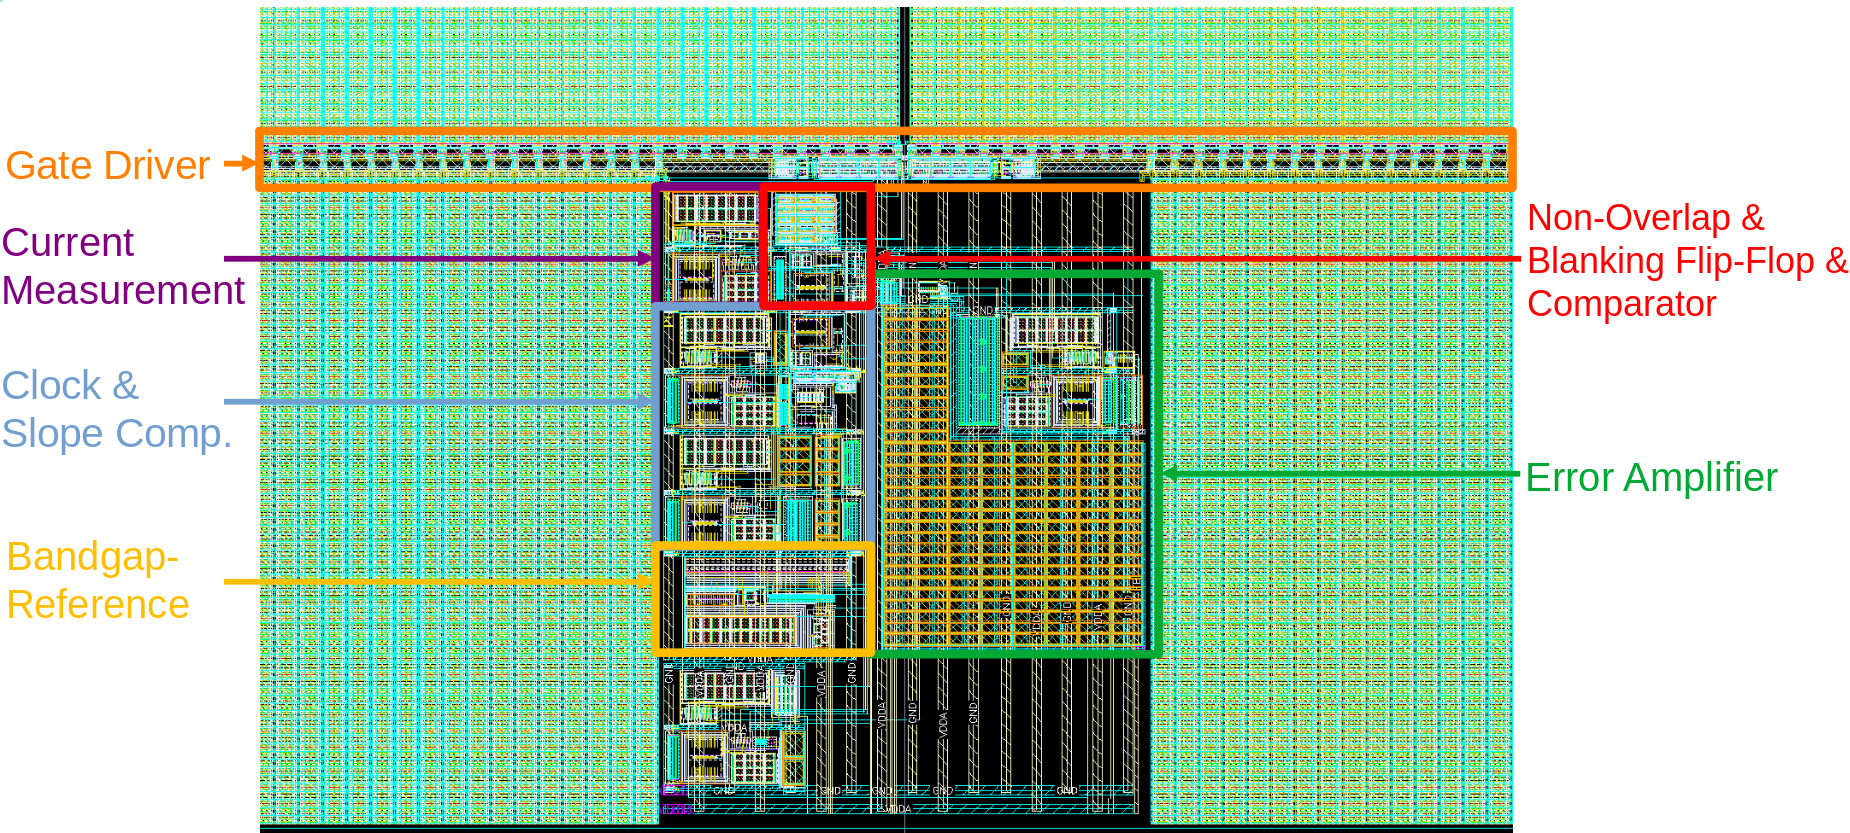
\includegraphics[width=1\textwidth]{../ASIC-DESIGN-2/images/07_DCDC/BuckBoostLayout.png}
    \caption{Layout of the buck-boost converter regulator surrounded by the large power stage transistors}
    \label{fig:BBlayout}
\end{figure}

\clearpage

\subsection{Overall Chip Floorplan}
As can be seen in \autoref{fig:chiplayout}, this design is significantly pad limited as opposed to core limited. The entire lower right corner is unused and in general the lower third is sparsely populated opposed the the upper two thirds which is entirely filled the the buck-boost converter. The large switching transistors were maximized to reduce conversions losses and take up the majority of the chips area. A large number of pads are used in parallel to meet our current handling capabilities and not exceed the recommendation of \qty{50}{\milli\ampere} per pad. In the bottom left the digital circuitry for the \ac{SPI} periphery and internal registers can be seen as well as supporting circuitry like the \ac{POR} and bandgap voltage reference. 
\begin{table}[H]
    \centering
    \begin{tabular}{|c|c|}
        Property & Value \\
        \hline
        Function & Buck-Boost Converter \\
        Package & QFN48 7x\qty{7}{\milli\meter} \\
        Process & X-Fab \qty{350}{\nano\meter} \\
		Size & \qty{2712}{\micro\meter} x \qty{2952}{\micro\meter} \\
        Area & \qty{8.006}{\milli\meter\squared}
    \end{tabular}
    \caption{ASIC Properties}
    \label{tab:spec_asic}
\end{table}
\begin{figure}[h]
    \centering
    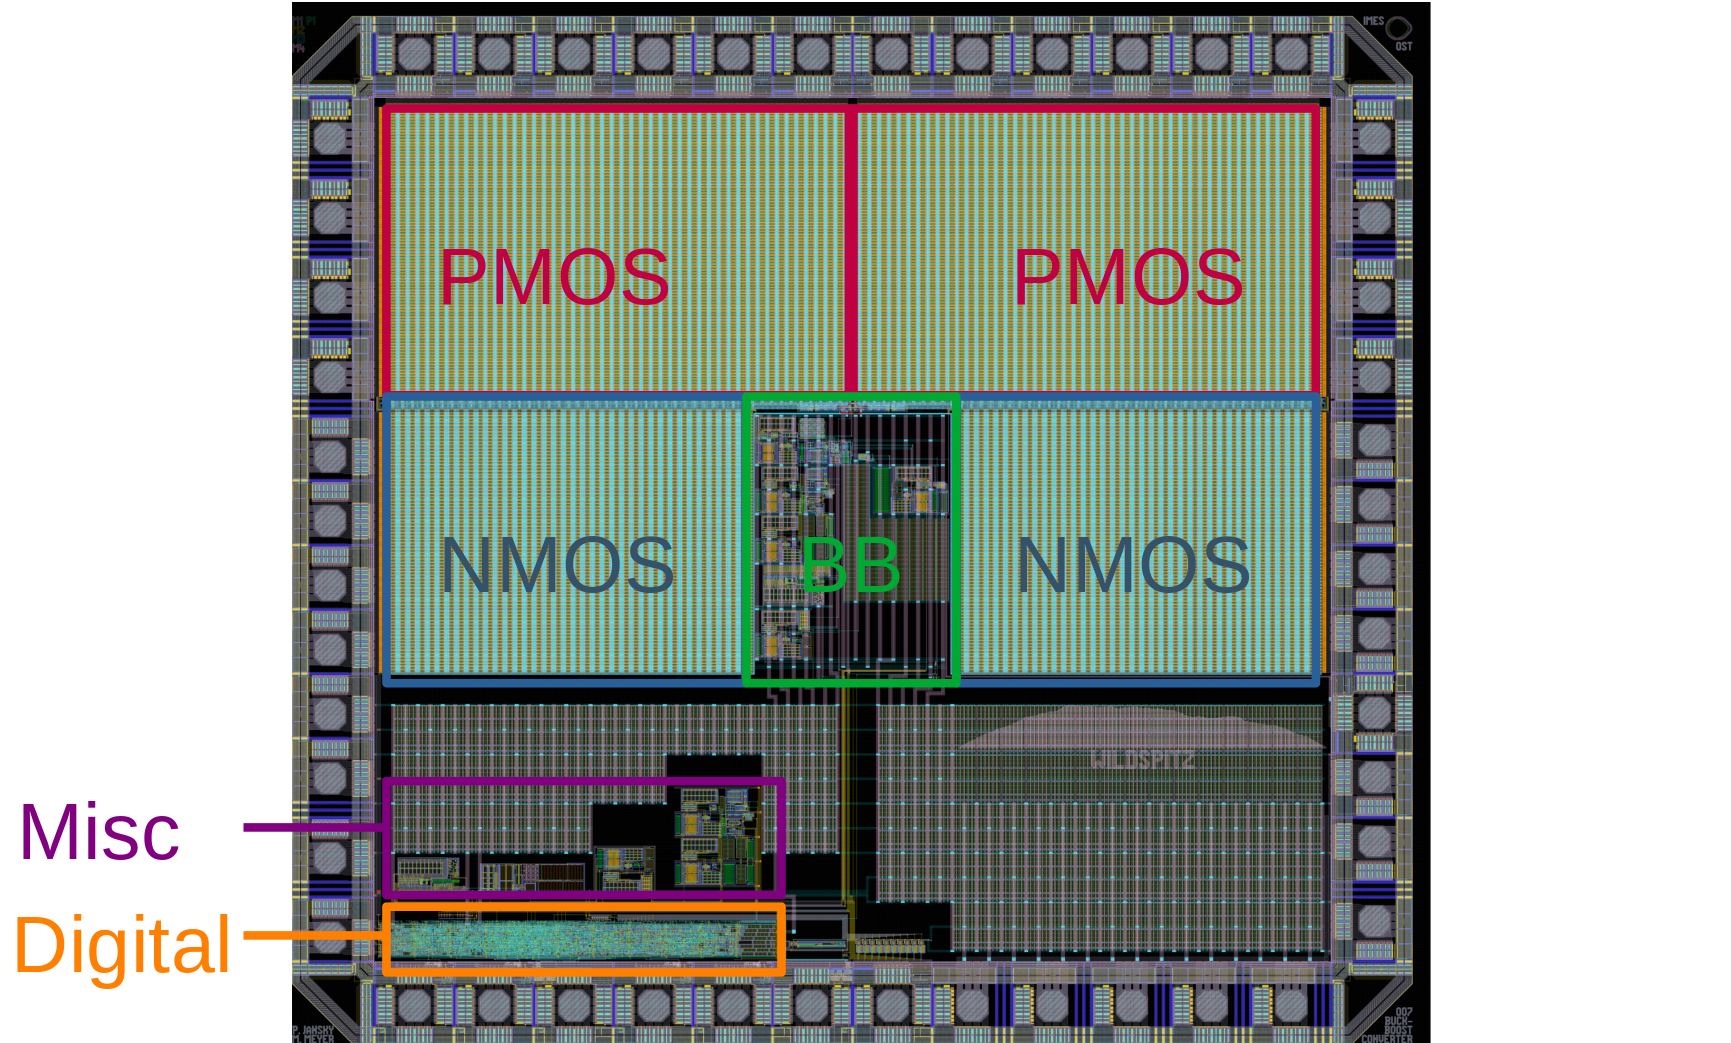
\includegraphics[width=1\textwidth]{../ASIC-DESIGN-2/images/07_DCDC/ChipLayout.png}
    \caption{Floorplan of the entire chip with annotations}
    \label{fig:chiplayout}
\end{figure}
\subsubsection{Package}
In \autoref{fig:package}, the package (QFN-48) of the chip is illustrated. It is evident that there are two distinct ground connections, namely GND and GND\_2, and two separate supply voltages, V\_IN and VDD\_D. These two domains can be interconnected on the Printed Circuit Board (PCB). However, to minimize noise interference and to facilitate separate analysis of the DC/DC converter and the rest of the circuit, these domains are not internally connected within the chip. Specifically, GND\_2 serves as the ground for the DC/DC converter, while GND is the ground for the digital part, bandgap, current reference, and so on. Similarly, V\_IN is the supply voltage for the DC/DC converter, and VDD\_D is the supply voltage for the remaining circuit components. 
\begin{figure}[h]
	\centering
	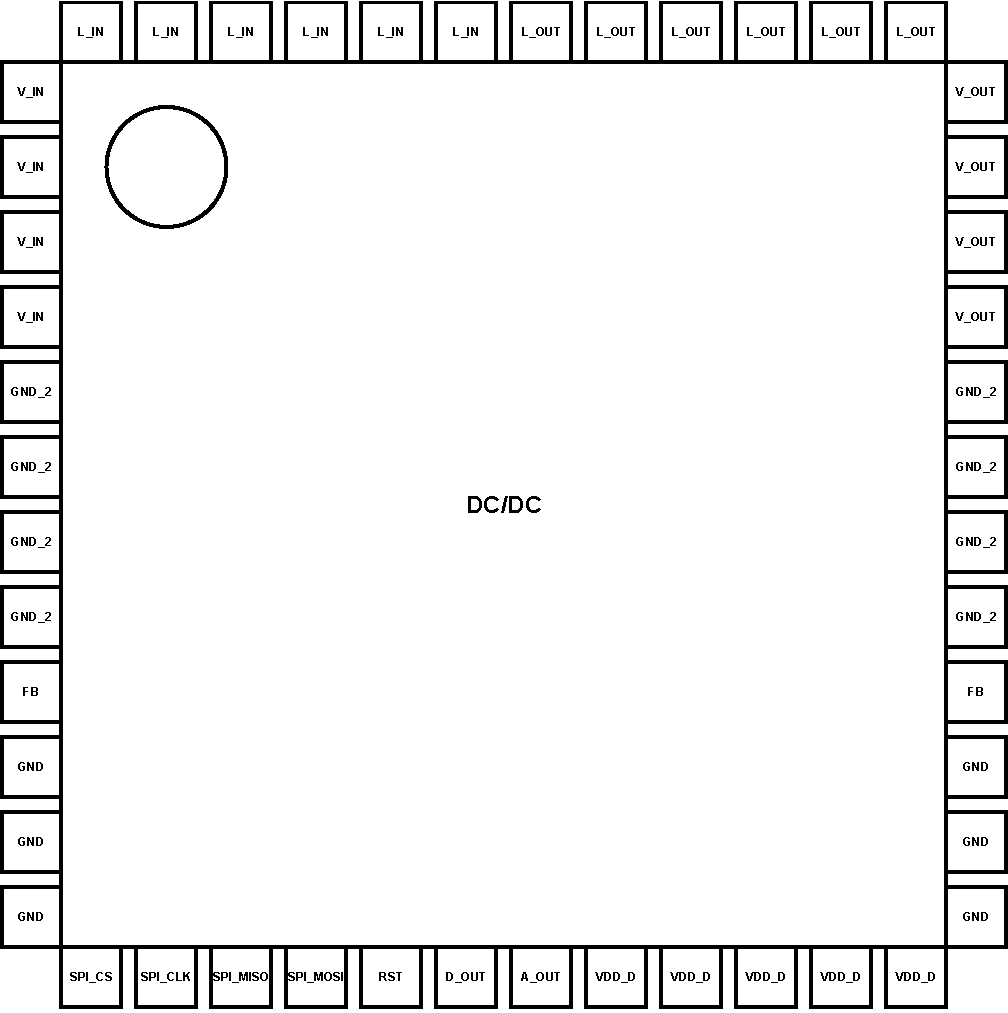
\includegraphics[width=1\textwidth]{../ASIC-DESIGN-2/images/pakage.pdf}
	\caption{Floor-plan Package, Top view}
	\label{fig:package}
\end{figure}

	% \section{Test Setup}

% \textcolor{red}{TBD}

	\section{Test Setup}
\label{sec:testsetup}
\subsection{Hardware}
\label{sec:hardware}
In this section we introduce the hardware setup we created in order to validate our chip design and compare the samples we received with the results we obtained from simulations. For an as like to like comparison as possible with the simulations we created hardware that replicates the virtual test bench setup as close as possible. The setup for instance contains electronically controllable loads like in the simulations to compare dynamic regulation characteristics of the buck-boost converter. These responses to load steps also give insight into the closed loop regulation characteristics like bandwidth and phase margin of the internal regulation loop. An additional goal is to verify our SPI slave implementation with a commercial SPI master device like an Arduino or USB to SPI converter. The accuracy of internal signals such as the internal oscillator and the the bandgap voltage reference are of additional interest. \\
List of intended measurements:
\begin{itemize}
    \item Line Regulation
    \item Load Regulation
    \item Output Voltage Regulation Accuracy 
    \item Efficiency
    \item Startup Behavior
    \item Short Circuit Behavior
    \item SPI Functionality
    \item Internal Oscillator Frequency Accuracy
    \item Bandgap Voltage Reference Accuracy
\end{itemize}

Going further with the test bench analogy, we split the test setup into two components, a test bench like PCB we call the Adapter PCB and multiple smaller PCBs which contain the \ac{DUT} we refer to as Hats, as they are socketed onto the Adapter PCB.


\subsubsection{Adapter PCB}
The main Adapter PCB contains the functionality of the test bench and has a common plug-in location for the \ac{DUT} containing Hats. The Adapter is designed in such a way, that the \ac{DUT} can be placed in the thermal chamber of the thermal airstream system TP04300A in order to test the \ac{DUT} functionality under various thermal conditions. Four electronically controllable load resistors are contained on the PCB for load step measurements and current sense amplifiers are used to measure the current flowing into and out of the switching converter. In order to verify the SPI communication with the \ac{DUT} we have included headers and voltage translators to connect with either an Arduino Nano Every or an FTDI FT232 based USB to SPI adapter.

\begin{figure}[h]
    \centering
    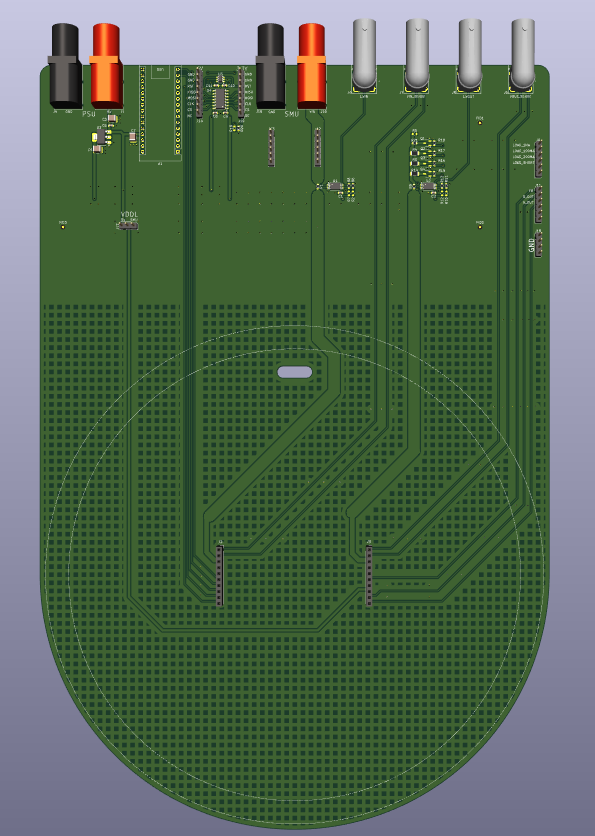
\includegraphics[width=0.6\textwidth]{../ASIC-DESIGN-2/images/02_test_setup/Adapter _PCB.png}
    \caption{3D render of the Adapter PCB}
    \label{fig:Adapter_PCB}
\end{figure}



\subsubsection{Hat PCB}
In total we created three Hat PCBs which can be used as \ac{DUT}s. One PCB contains a commercially available IC and we created two PCBs for our manufactured chip. In the first PCB our chip is placed into an \ac{IC} socket and in the second one the QFN package soldered directly to the board. The socketed version allows for the quick characterization of multiple chips and measurement of the variance of characteristics over the samples. The socket however introduces higher lead resistances and inductances as well as thermally isolates the chip from the PCB. The thermal isolation could lead to increased temperatures in high load conditions and in a worst case scenario could lead to damage of the chip. We did not expect these factors to play a major role, but out of caution we decided design the soldered version as a fallback. During testing we did not observe a measurable difference in characteristics based on if the chip was socketed or not.\\


\begin{figure}[h]
    \centering
    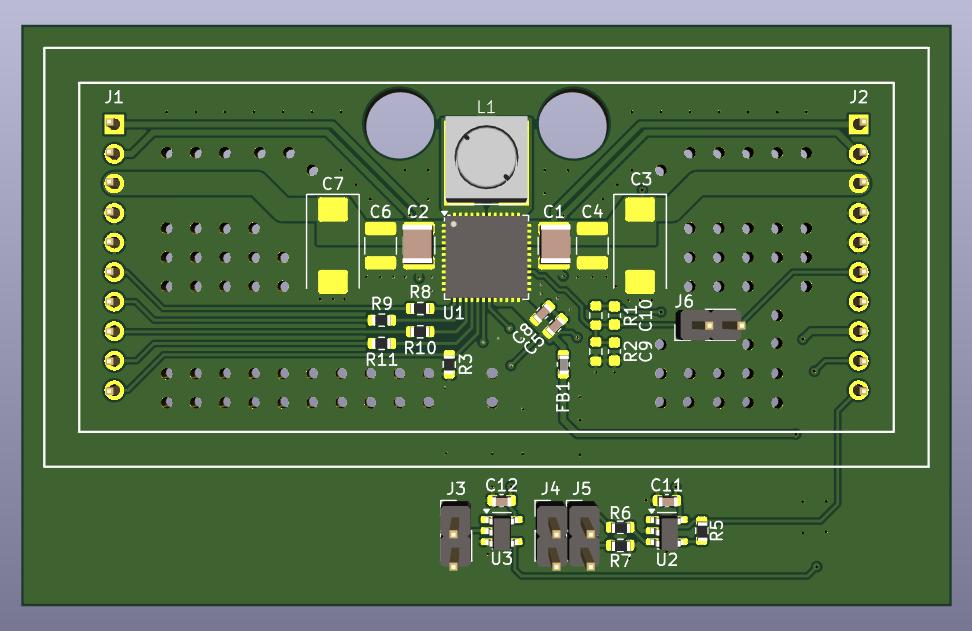
\includegraphics[width=0.8\textwidth]{../ASIC-DESIGN-2/images/02_test_setup/ASIC_Hat_PCB.png}
    \caption{3D render of the Hat PCB with the QFN package soldered to the PCB}
    \label{fig:ASIC_Hat}
\end{figure}


Our reasoning to create a Hat with a commercially available chip was two fold. First it allows validation of the test setup with a real hardware \ac{DUT} before receiving samples and secondly creates a baseline to compare our design against. For the commercially available \ac{IC} we used the TPS63900 from Texas Instruments. While this \ac{IC} is significantly smaller in physical size, it has a similar input and voltage range as well as current drive capabilities. Similarly it is also a highly integrated buck-boost converter with integrated switches in the standard cascaded-buck-boost converter topology. The TPS63900 however has a significantly higher efficiency, greater than \qty{90}{\percent}\cite{tps63900}, as it is designed for ultra low power applications and implements multiple advanced power saving features like dynamic switching frequency adjustment based on load conditions\cite{tps63900}. They additionally employ a novel drive scheme of the power stage leading to trapezoidal inductor current, as opposed to the traditional triangular waveform, which again leads to higher efficiency and to only a single operating mode over the entire input and output voltage range\cite{tps63900}. 
	

\subsection{Software}

\subsubsection{Architecture}
For the architecture of the test software, it was decided to adopt a modular approach with separate classes for each test and measurement instrument. This architecture facilitates easy extension of the software with new instruments and tests. Additionally, it allows looping over different tests without the need to initialize and close measurement instruments every time they are used. For data storage, the decision was made to employ a database, as it offers a convenient way to store and analyze data afterward. Thereby SQLite was chosen as the database solution due to its lightweight nature and ease of use, requiring no server to be running. The database was structured with the following columns:
\begin{itemize}
    \item \textbf{Id}: The unique identifier for each measurement.
    \item \textbf{chip\_id}: The identifier for the chip that was measured.
    \item \textbf{measurement\_type}: The type of measurement performed.
    \item \textbf{parameter1}: The first parameter used for the test, such as the input voltage applied.
    \item \textbf{parameter2}: The second parameter used for the test, such as the load applied to the output.
    \item \textbf{temperature}: The temperature of the chip during the measurement.
    \item \textbf{data}: The measured data.
    \item \textbf{measurement\_result}: The result of the measurement, if applicable.
    \item \textbf{Timestamp}: The timestamp of the measurement.
\end{itemize}

\subsubsection{Test Software Language}
The test software was implemented using Python. Python is a high-level programming language widely utilized in the scientific community and increasingly in testing due to its ease of learning and the availability of drivers for nearly every measurement instrument\cite{Wikipedia:Python}. Additionally, one of the authors had prior experience in writing test scripts in Python for chip verification and validation, enabling the initiation of test writing without a significant investment in learning a new programming language and environment.

\subsubsection{Test Software Implementation}
Prior to commencing the test software development, the various tests to be performed were determined, aiming to align with those conducted in simulations. These included:
\begin{itemize}
    \item Startup behavior with reset disabled.
    \item Startup behavior with active reset and subsequently disabled reset.
    \item Load step response with load variations of 10mA, 100mA, and 200mA.
    \item Output response to stepped input voltage changes.
    \item Turn-off and turn-on behavior with brief reset enablement.
    \item SPI test to mux out the wanted analog/digital signal, change the clock frequency, and read back the register values.
\end{itemize}

\subsubsection{Test Setup}
The primary test setup utilized the PXI system from National Instruments (NI). This system integrates various measurement instruments into a single unit and serves as the computer running the Python code. Consequently, there are minimal delays due to additional wires between the computer and measurement instruments. Moreover, synchronized triggers are available on this measurement system, eliminating the need for trigger wiring between instruments. This advantage reduces setup complexity and wiring requirements. The specific PXI system employed was the PXI model \glqq{}NI PXIe-8881\grqq{}, equipped with the following modules:

\begin{itemize}
    \item \textbf{PXIe-4141}: This is a SMU (Source Measurement Unit) which can be used to apply the input voltage to the chip.
    \item \textbf{E3631A}: This is a power supply which can be used to apply the input voltage to the chip.
    \item \textbf{PXI-5142}: This is a two channel oscilloscope used to measure the output and input voltage of the chip.
    \item \textbf{PXI-5163}: This is a two channel oscilloscope used to measure the output and input current of the chip.
    \item \textbf{TP04300}: This is the thermostreamer used to control the temperature of the chip.
    \item \textbf{PXI-6363}: This is a GPIO controller used to control the reset of the chip and the different load resistors.
    \item \textbf{NGE-100}: This is a power supply to provide the power for the test circuit.
    \item \textbf{FTDI C232HM-DDHSL-0}: This is a USB to SPI converter used to communicate with the chip.
\end{itemize}

An overview of all the instruments can be seen in Figure \autoref{fig:overview}. More details about the hardware can also be found in the \href{https://github.com/gstei/asic_validation/}{git repository}\footnote{https://github.com/gstei/asic\_validation.git} where test was written.

\begin{figure}[h]
    \centering
    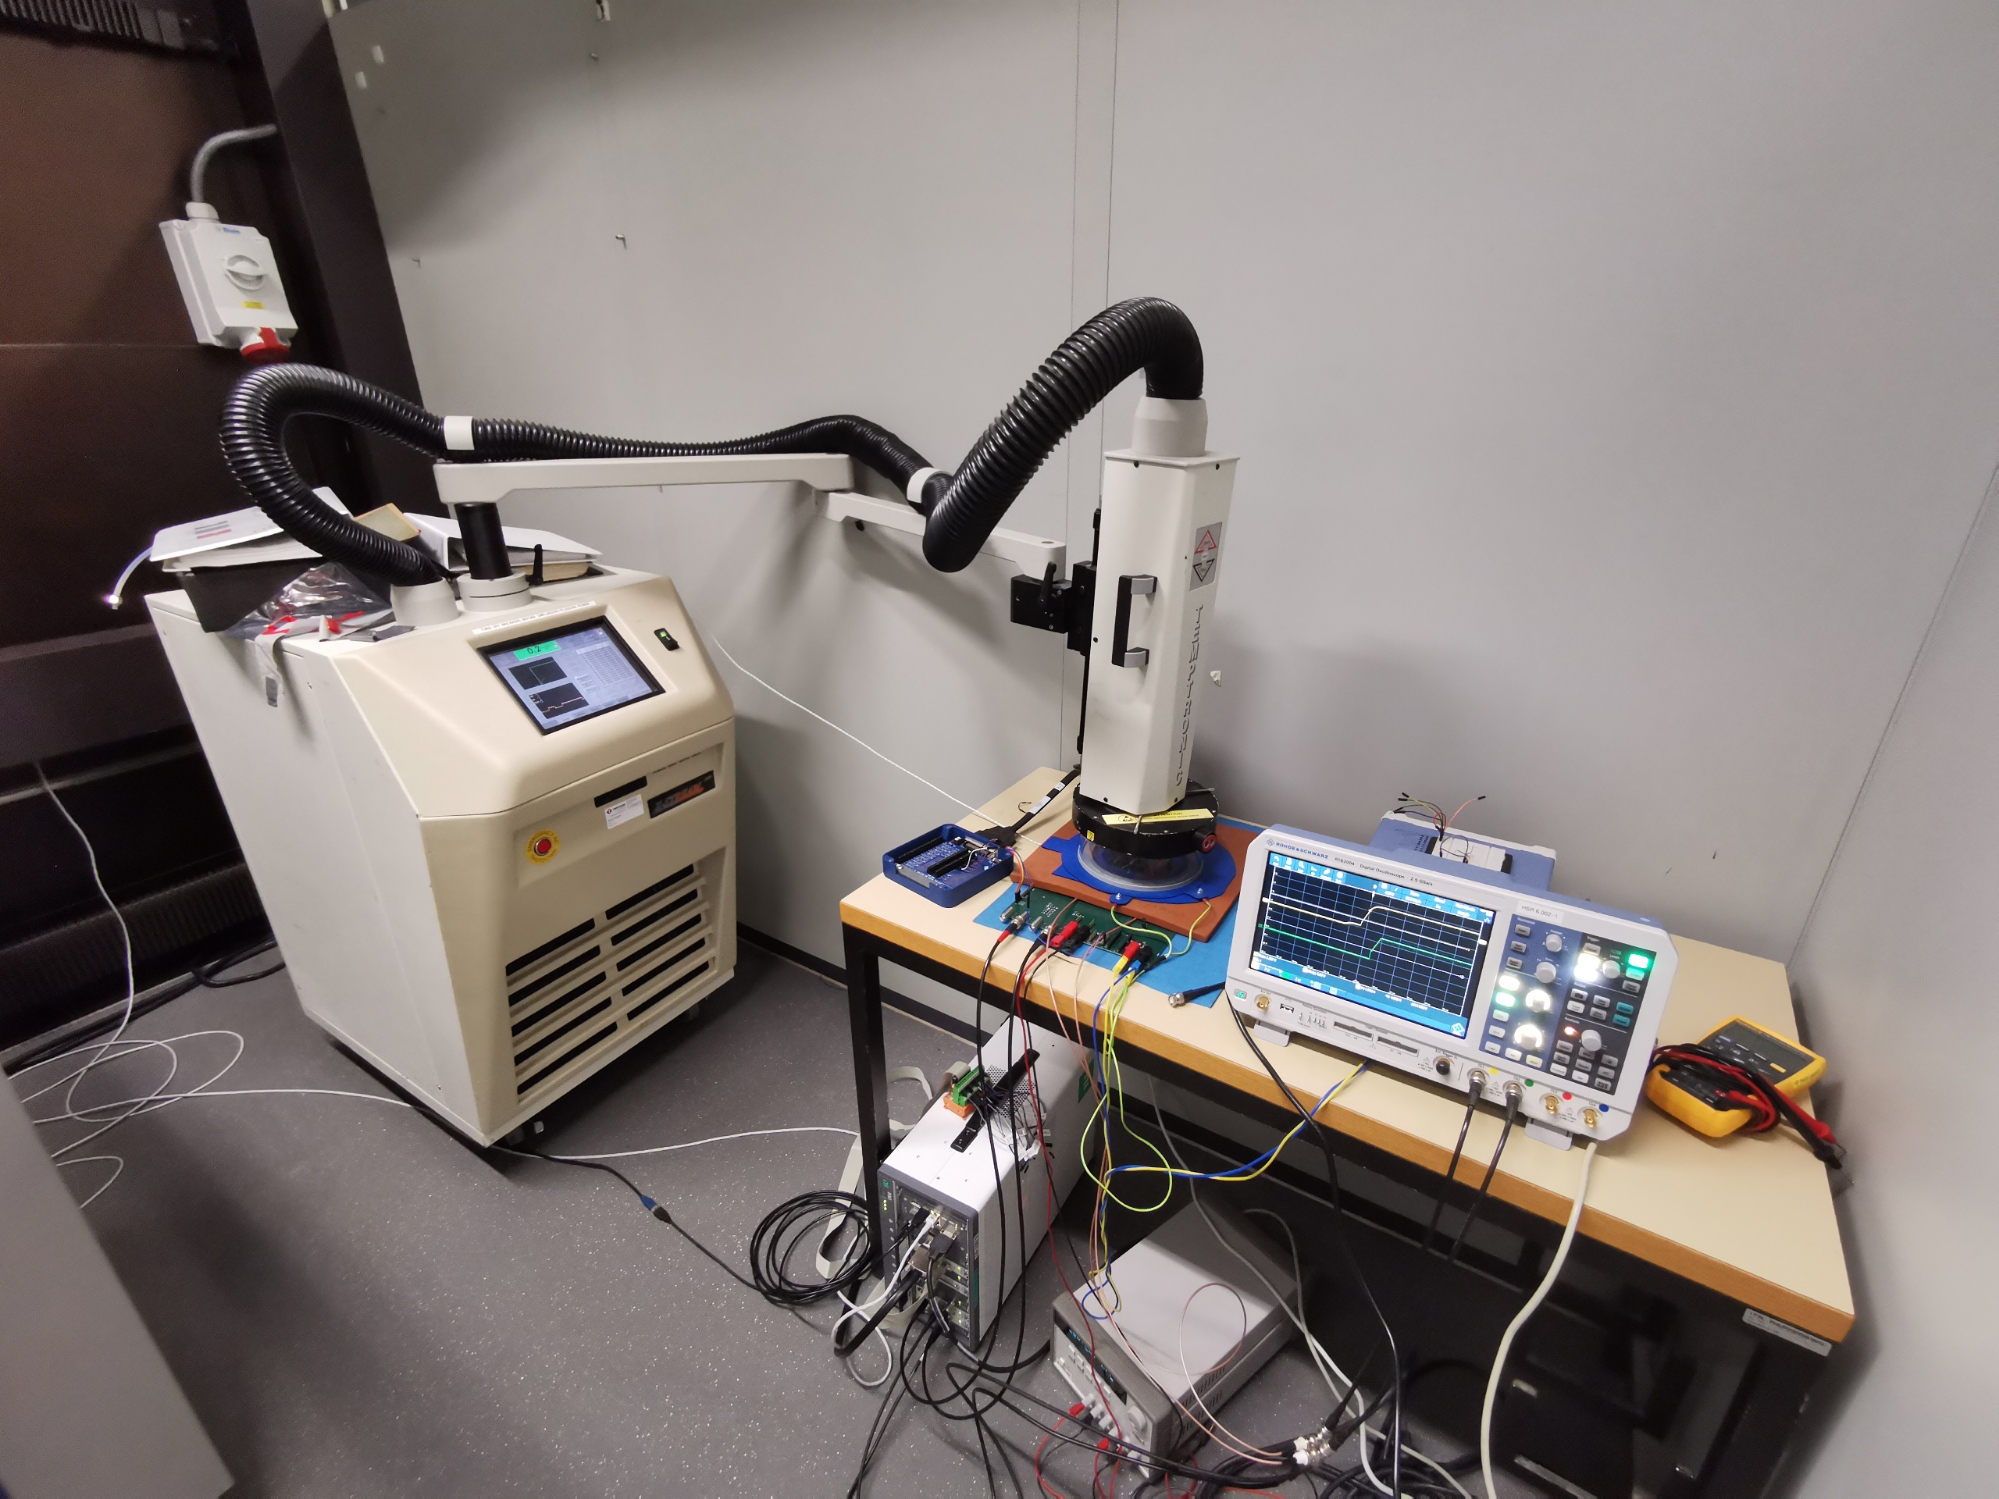
\includegraphics[width=0.8\textwidth]{../ASIC-DESIGN-2/images/02_test_setup/01_overview.jpg}
    \caption{Overview of the test setup}
    \label{fig:overview}
\end{figure}

\subsubsection{Github}
The test software was written using Git as its version control system, with the repository being hosted on GitHub. This choice was driven by GitHub's widespread adoption and its seamless integration for collaborative code sharing among team members. Furthermore, Git's robust features allow for efficient tracking of changes and management of various software versions. The repository can be found at \href{https://github.com/gstei/asic_validation.git}{the following link}\footnote{https://github.com/gstei/asic\_validation.git}. Furthermore the repository uses github actions to automatically run tests on every push to the repository. This ensures that the code is written in a nice way according to the PEP8 standard and that the tests are most probably running without any errors, for that \href{par:Flake8}{flake8} and \href{par:Pylint}{pylint} were used as linter and integrated in the github workflow.

\paragraph{Pylint}
\label{par:Pylint}
Pylint is a static code analysis tool for Python, adhering to the style guidelines outlined in PEP 8. It checks various aspects of Python code, including line length, variable naming conventions, and interface implementation consistency. Pylint is similar to Pychecker and Pyflakes but offers additional features such as generating UML diagrams using the Pyreverse module. It can be used independently or integrated into various IDEs and editors like Eclipse with PyDev, Spyder, Visual Studio Code, Atom, GNU Emacs, and Vim\cite{Wikipedia:Pylint}.

\paragraph{Flake8}
\label{Par:Flake8}
Flake8 is a Python linting tool that scans Python codebases for errors, style inconsistencies, and complexity. It consists of three underlying tools: PyFlakes for error checking, McCabe for complexity analysis, and pycodestyle for style conformity with PEP8 guidelines. Flake8 stands out due to its extensive plugin ecosystem, allowing users to augment its capabilities and address a wide range of issues and concerns in Python code\cite{flake8}.


\subsubsection{SPI Interface}
\label{subsubsec:SPI}
The registers of the chip can be controlled over a SPI interface, therefore a SPI Master was needed.
It was decided to implemented the SPI master using the FTDI C232HM-DDHSL-0 USB to SPI converter. The FTDI chip was chosen due to its ease of use and the availability of drivers for Python. But it finally turned out that the SPI mode 1 which was implemented on the chip does not exactly correspond to SPI mode 1 implemented on the FTDI Chip. On the FTDI Chip the CS and the first SPI clock edge are turned on on the same time, but on the test bench used in the simulation to verify the digital part of the chip this was not the case and due to its implementation the finite state machine only works when the CS is turned on before the first clock edge as it is also visible in \autoref{fig:spi_modes} (CPOL=0, CPHA=1). Therefore a custom driver was implemented in software which only works at 1kHz instead of 500kHz, but since one only needs to write eight different register this does not really matter. Since the human counterpart does not see the difference. Nevertheless for further projects we would recommend to have a look at the test instruments already when designing the chip to avoid such problems. Nevertheless the SPI interface should work with a normal micro controller which uses the SPI standard as as it can be seen in \autoref{fig:spi_modes} where the CS is turned on before the first clock edge. Nevertheless there are some special implementations of the SPI as in the FTDI C232HM-DDHSL-0 which should have been covered as well during the design.
\begin{figure}[h]
    \centering
    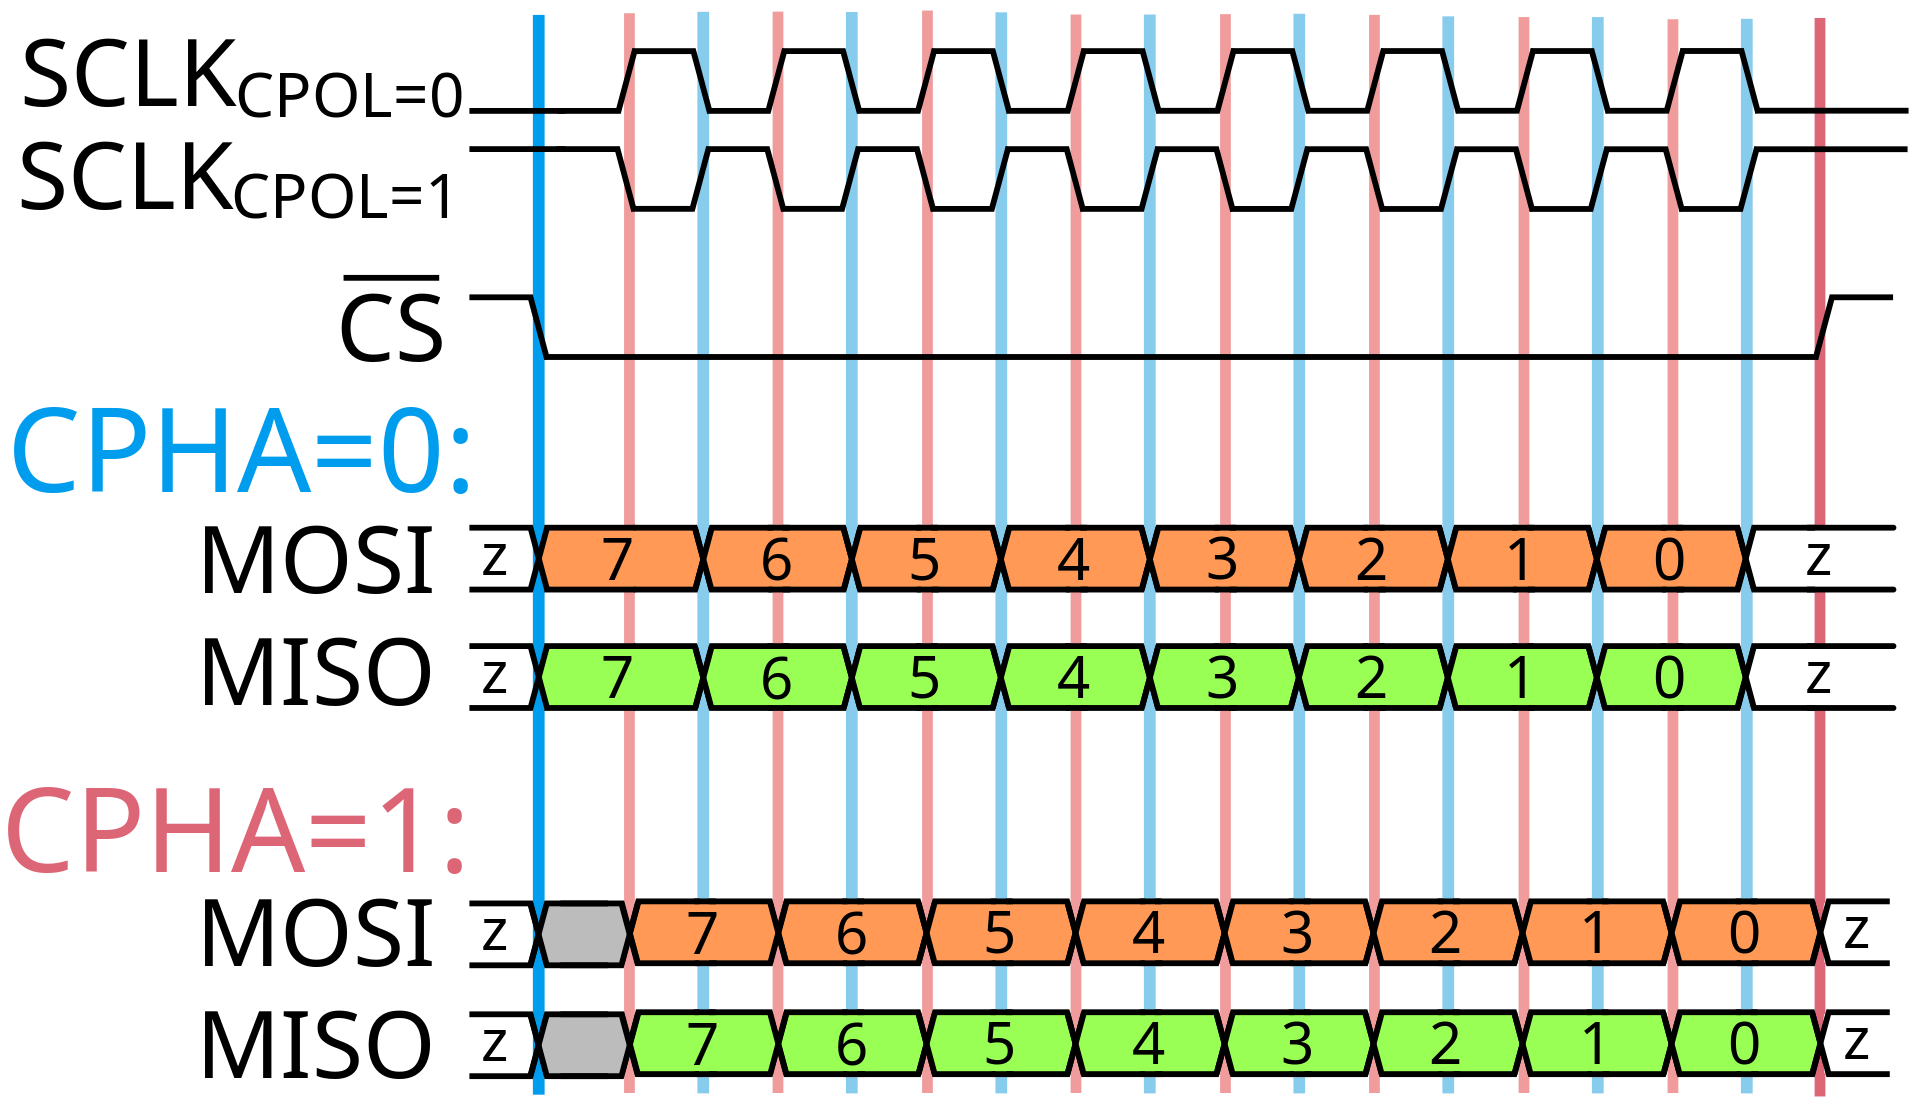
\includegraphics[width=0.8\textwidth]{../ASIC-DESIGN-2/images/04_spi/SPI_timing_diagram_CS.svg.png}
    \caption{SPI Modes \cite{Wikipedia:SPI}}
    \label{fig:spi_modes}
\end{figure}
\subsubsection{Conclusion}
In retrospective one can say that it was a very good decision to spend quite some time in the software architecture in the beginning of the project and to use a database. Since it turned out that once it is clear what and how something has to be implemented the software can be written quite fast and with the code checker in the background also with a reasonable quality, this for example allowed to add the thermostreamer to the tests within two hours without any issues and all measurement results were available in the database. Nevertheless it also turned out that when the chip does not behave as expected the test script is not useful at all. Due to that the automated tests only worked with the TI chip, but not with our chip since we had startup problems on our chip which caused that the whole automated test could not be executed since the chip started not correctly as also mentioned in 
\autoref{subsubsec:cur_mes_inac}.


	
	
	\section{Results}
\label{sec:results}
On the SPI interface one should be able to successfully write and read back registers. Therefore a complete SPI driver was written in python which allows to simply mux out the wanted analog/digital signal, change the clock frequency and read back the register values. An overview of the registers can be found bellow whereby register 7 is not connected to anything and therefore not listed in \autoref{tab:reg_des}.
\subsection{SPI Interface}
\begin{longtable}{|p{3.5cm}|p{10.5cm}|}
	\hline
	\rowcolor{lightgray}
	\textbf{Register Number} &\textbf{Function} \\ \hline
	0 & stores the last spi command $<7:0>$\\ \hline
    1 & read only register with following value: b0=1, b1=0, b2=1, b3=0, b4=0, b5=0, b6=0, b7=0 <15:8> \\ \hline
    3 & analog mux $<20:16>$ 0=ground, 1=iboot ref, 2=vbgp, 3=output error amplifier, 4=ground,  5= ground \\ \hline
	4 & current limit tune $<27:25>$, current limit tune enable $<24>$ \\ \hline
	5 & output voltage fb $<32>$ \\ \hline
	6 & Freq tune digital part $<42:40>$ can add up to 3 caps eq sized caps to saw tooth ==> clock 4 times slower, dig out$<47>$ ==> enable clock on digital pad\\ \hline
    7 & Freq tune linear regulator$<50:48>$ can add up to 3 caps eq sized caps to saw tooth ==> clock 4 times slower \\ \hline
	\caption{Register description} % needs to go inside longtable environment
	\label{tab:reg_des}
\end{longtable}
Since the the SPI communication is working as in the testbench and the testscript is available in the git repository. No further test results are listed here. But one thing that one has to be aware of when one wants to control the chip is that the CS line has to be activated before the first clock edge arrives otherwise the communication will not work as mentioned in \autoref{subsubsec:SPI}.

\subsection{POR}
According to the simulation, the power-on reset (POR) exhibits the characteristics depicted in \autoref{tab:por}. The POR measurement was conducted on a single random sample at room temperature. To measure the characteristics from the simulation, a pull-up resistor was connected to the output of the analog test pin as the test pin exhibits high impedance when the chip is unpowered and is grounded when the chip is powered (as long as the analog test pint was not configured differently over the SPI).
Consequently, when the chip gets powered and reaches a voltage over the minimum voltage of the POR, the analog test pin is driven to zero and this change is observable. Due to that it turned out that the minimum voltage of the POR is \qty{3.72}{\volt} which is \qty{0.02}{\volt} more than the upper corner of the Simulation. Since the time was limited and the deviation is very small no further investigations were made on that. The input and output delay where measured the same way and it turned out that those values are inside the corners of the simulations. For the input delay a value of \qty{40}{\micro\second} was measured which is the time from which the input voltage is over over  \qty{3.72}{\volt} and the analog test pin is driven to ground. The other way around a value of \qty{6.5}{\micro\second} was measured as it can be also seen in \autoref{tab:por} column four.
\begin{longtable}{|p{2.5cm}|p{2.5cm}|p{2.5cm}|p{2.5cm}|p{2.5cm}|}
	\hline
	\rowcolor{lightgray}
	\textbf{Description} &\textbf{Min.} &\textbf{Max.} & \textbf{Mes.} & \textbf{Unit} \\ \hline
	
	input delay & 26 & 44 & 40  &\qty{}{\micro\second} \\ \hline
	output delay & 4.4 & 6.8 & 6.5 &\qty{}{\micro\second} \\ \hline
	Current consumption & 13 & 31 & -& \qty{}{\micro\ampere} \\ \hline
	Min voltage & 3.176& 3.7 & 3.72 & \qty{}{\volt} \\ \hline
	\caption{POR characteristic} % needs to go inside longtable environment
	\label{tab:por}
\end{longtable}
\subsection{Bandgap}
\label{subsubsec:bandgap}
The bandgap characteristics from the simulation can be seen in \autoref{tab:bandgap}, \autoref{fig:bandgap_voltage_vs_temp} and \autoref{fig:bandgap_voltage_mc}. The measurements have thereby shown that the bandgap voltage is in the range of of the simulation, the mean value is just shifted by 10mV. As it can be seen in the comparison of \autoref{fig:bandgap_voltage_distrb} and \autoref{fig:bandgap_voltage_mc}. Furthermore due to the fact that the reference current is slightly to high the center of the bandgap vs temperature curve is not anymore at \qty{40}{\degreeCelsius} but at about \qty{55}{\degreeCelsius} as it can be seen in the comparison of \autoref{fig:bandgap_voltage_vs_temp} and \autoref{fig:bandgap_voltage_vs_temp_mes}. About the other parameters like the current consumption and the min voltage no measurements could be done since the band gap is not directly accessible.
\begin{longtable}{|p{3.5cm}|p{3.5cm}|p{3.5cm}|p{3.5cm}|}
	\hline
	\rowcolor{lightgray}
	\textbf{Description} &\textbf{Min} &\textbf{Max} & \textbf{Unit} \\ \hline
	
	Bandgap voltage & 1.226 & 1.277 &\qty{}{\volt} \\ \hline
	Current consumption & 16.73 & 23.53 & \qty{}{\micro\ampere} \\ \hline
	Min voltage & 2.3& 2.9 & \qty{}{\volt} \\ \hline
	\caption{Bandgap characteristic} % needs to go inside longtable environment
	\label{tab:bandgap}
\end{longtable}
\begin{figure}[ht]
	\centering
	\includegraphics[width=\textwidth]{images/05_bandgap/band_volt.pdf}
	\caption{Bandgap voltage vs temperature simulated}
	\label{fig:bandgap_voltage_vs_temp}
\end{figure}
\begin{figure}[ht]
	\centering
	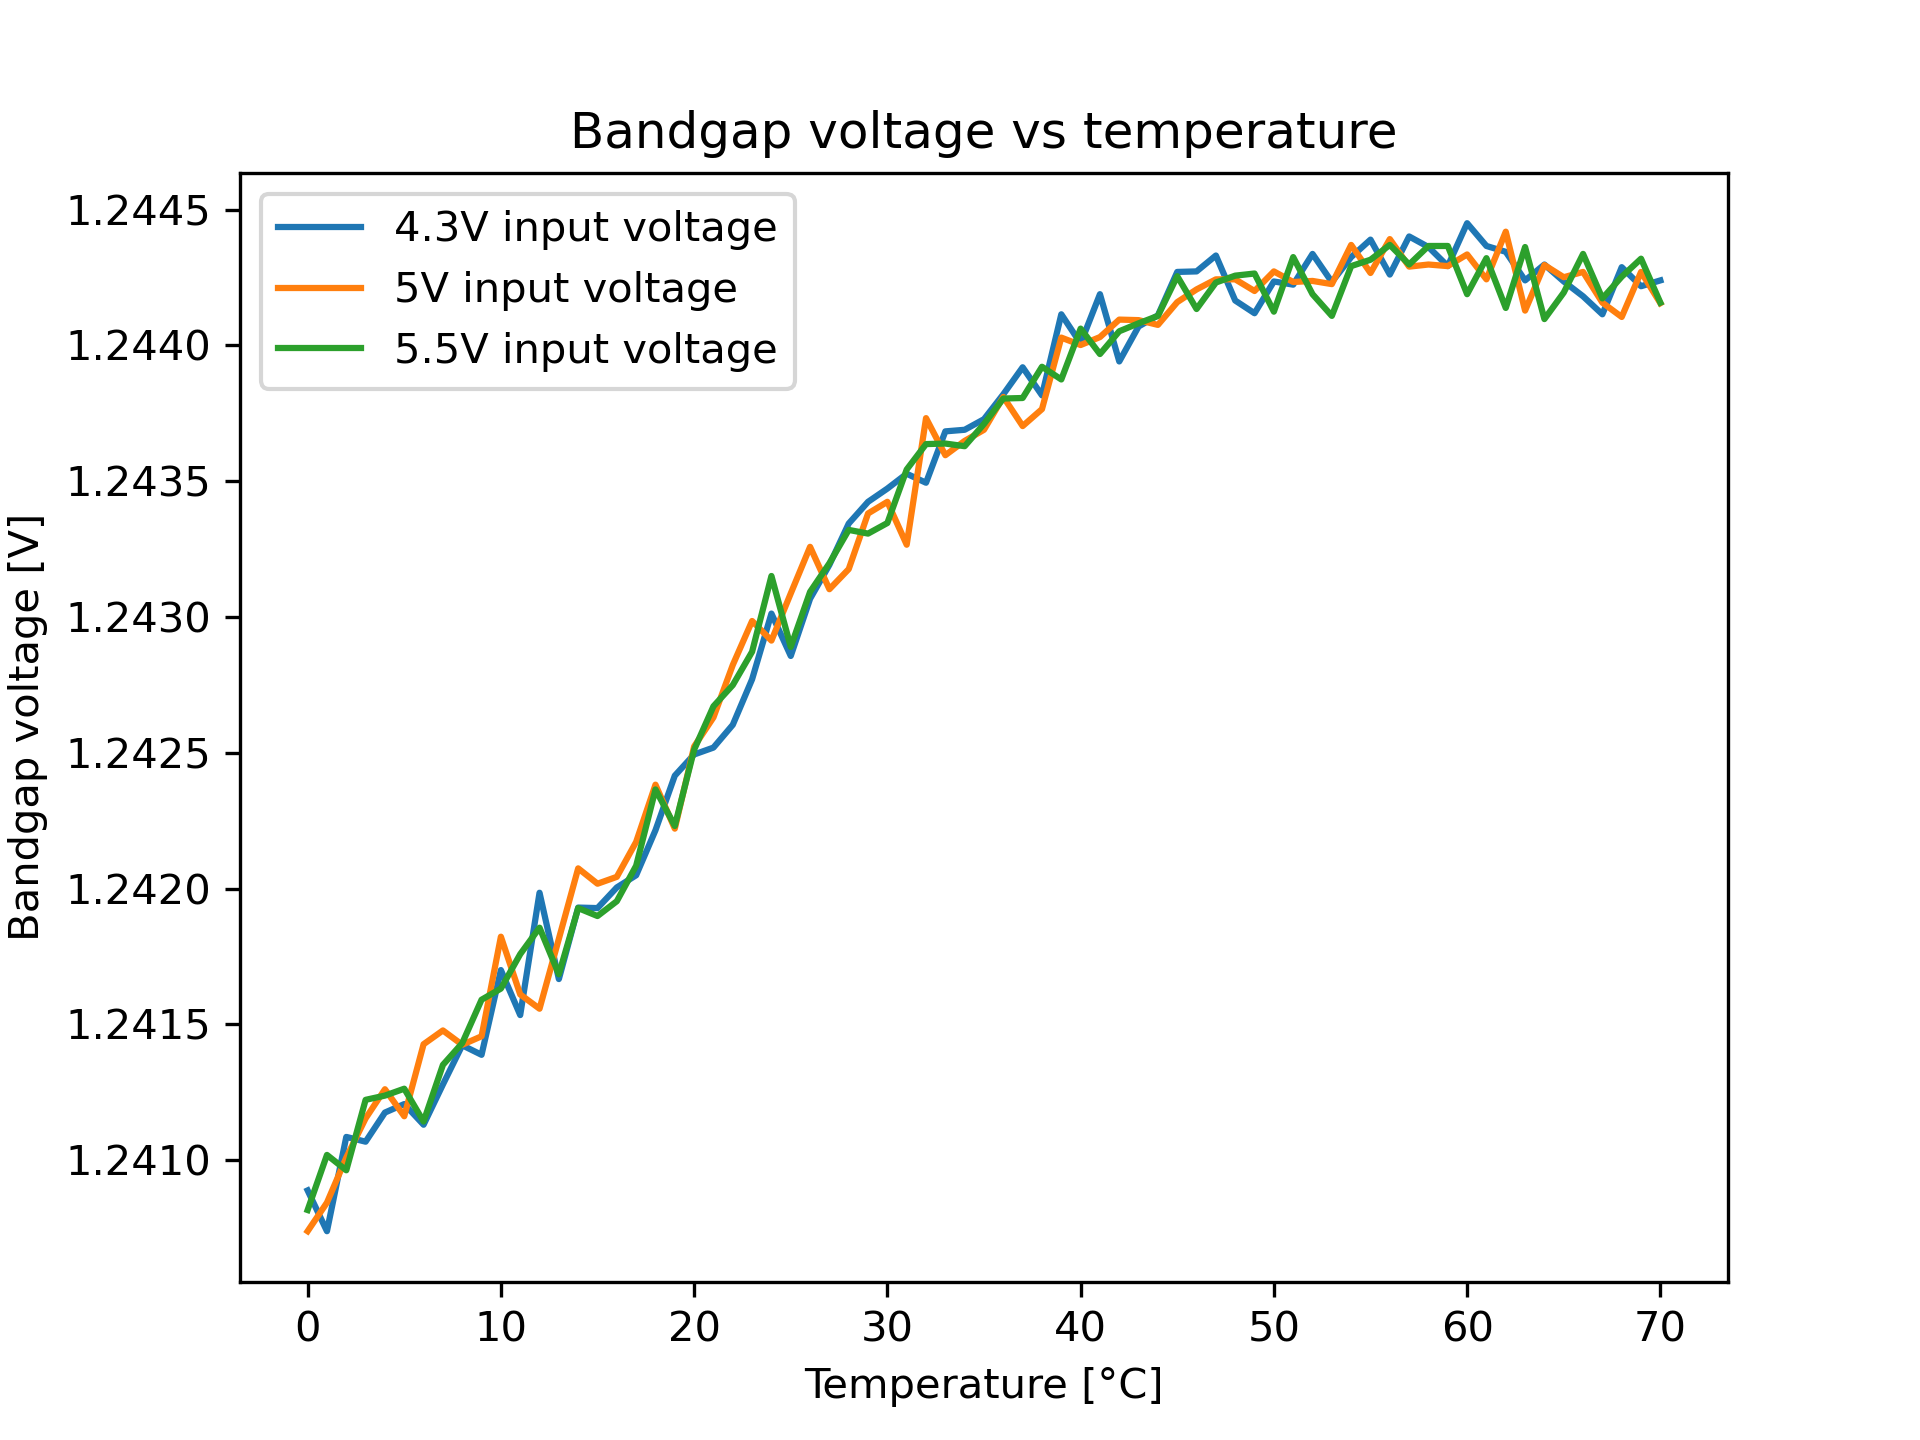
\includegraphics[width=\textwidth]{images/05_bandgap/Bandgap.png}
	\caption{Bandgap voltage vs temperature measured}
	\label{fig:bandgap_voltage_vs_temp_mes}
\end{figure}
\begin{figure}[ht]
	\centering
	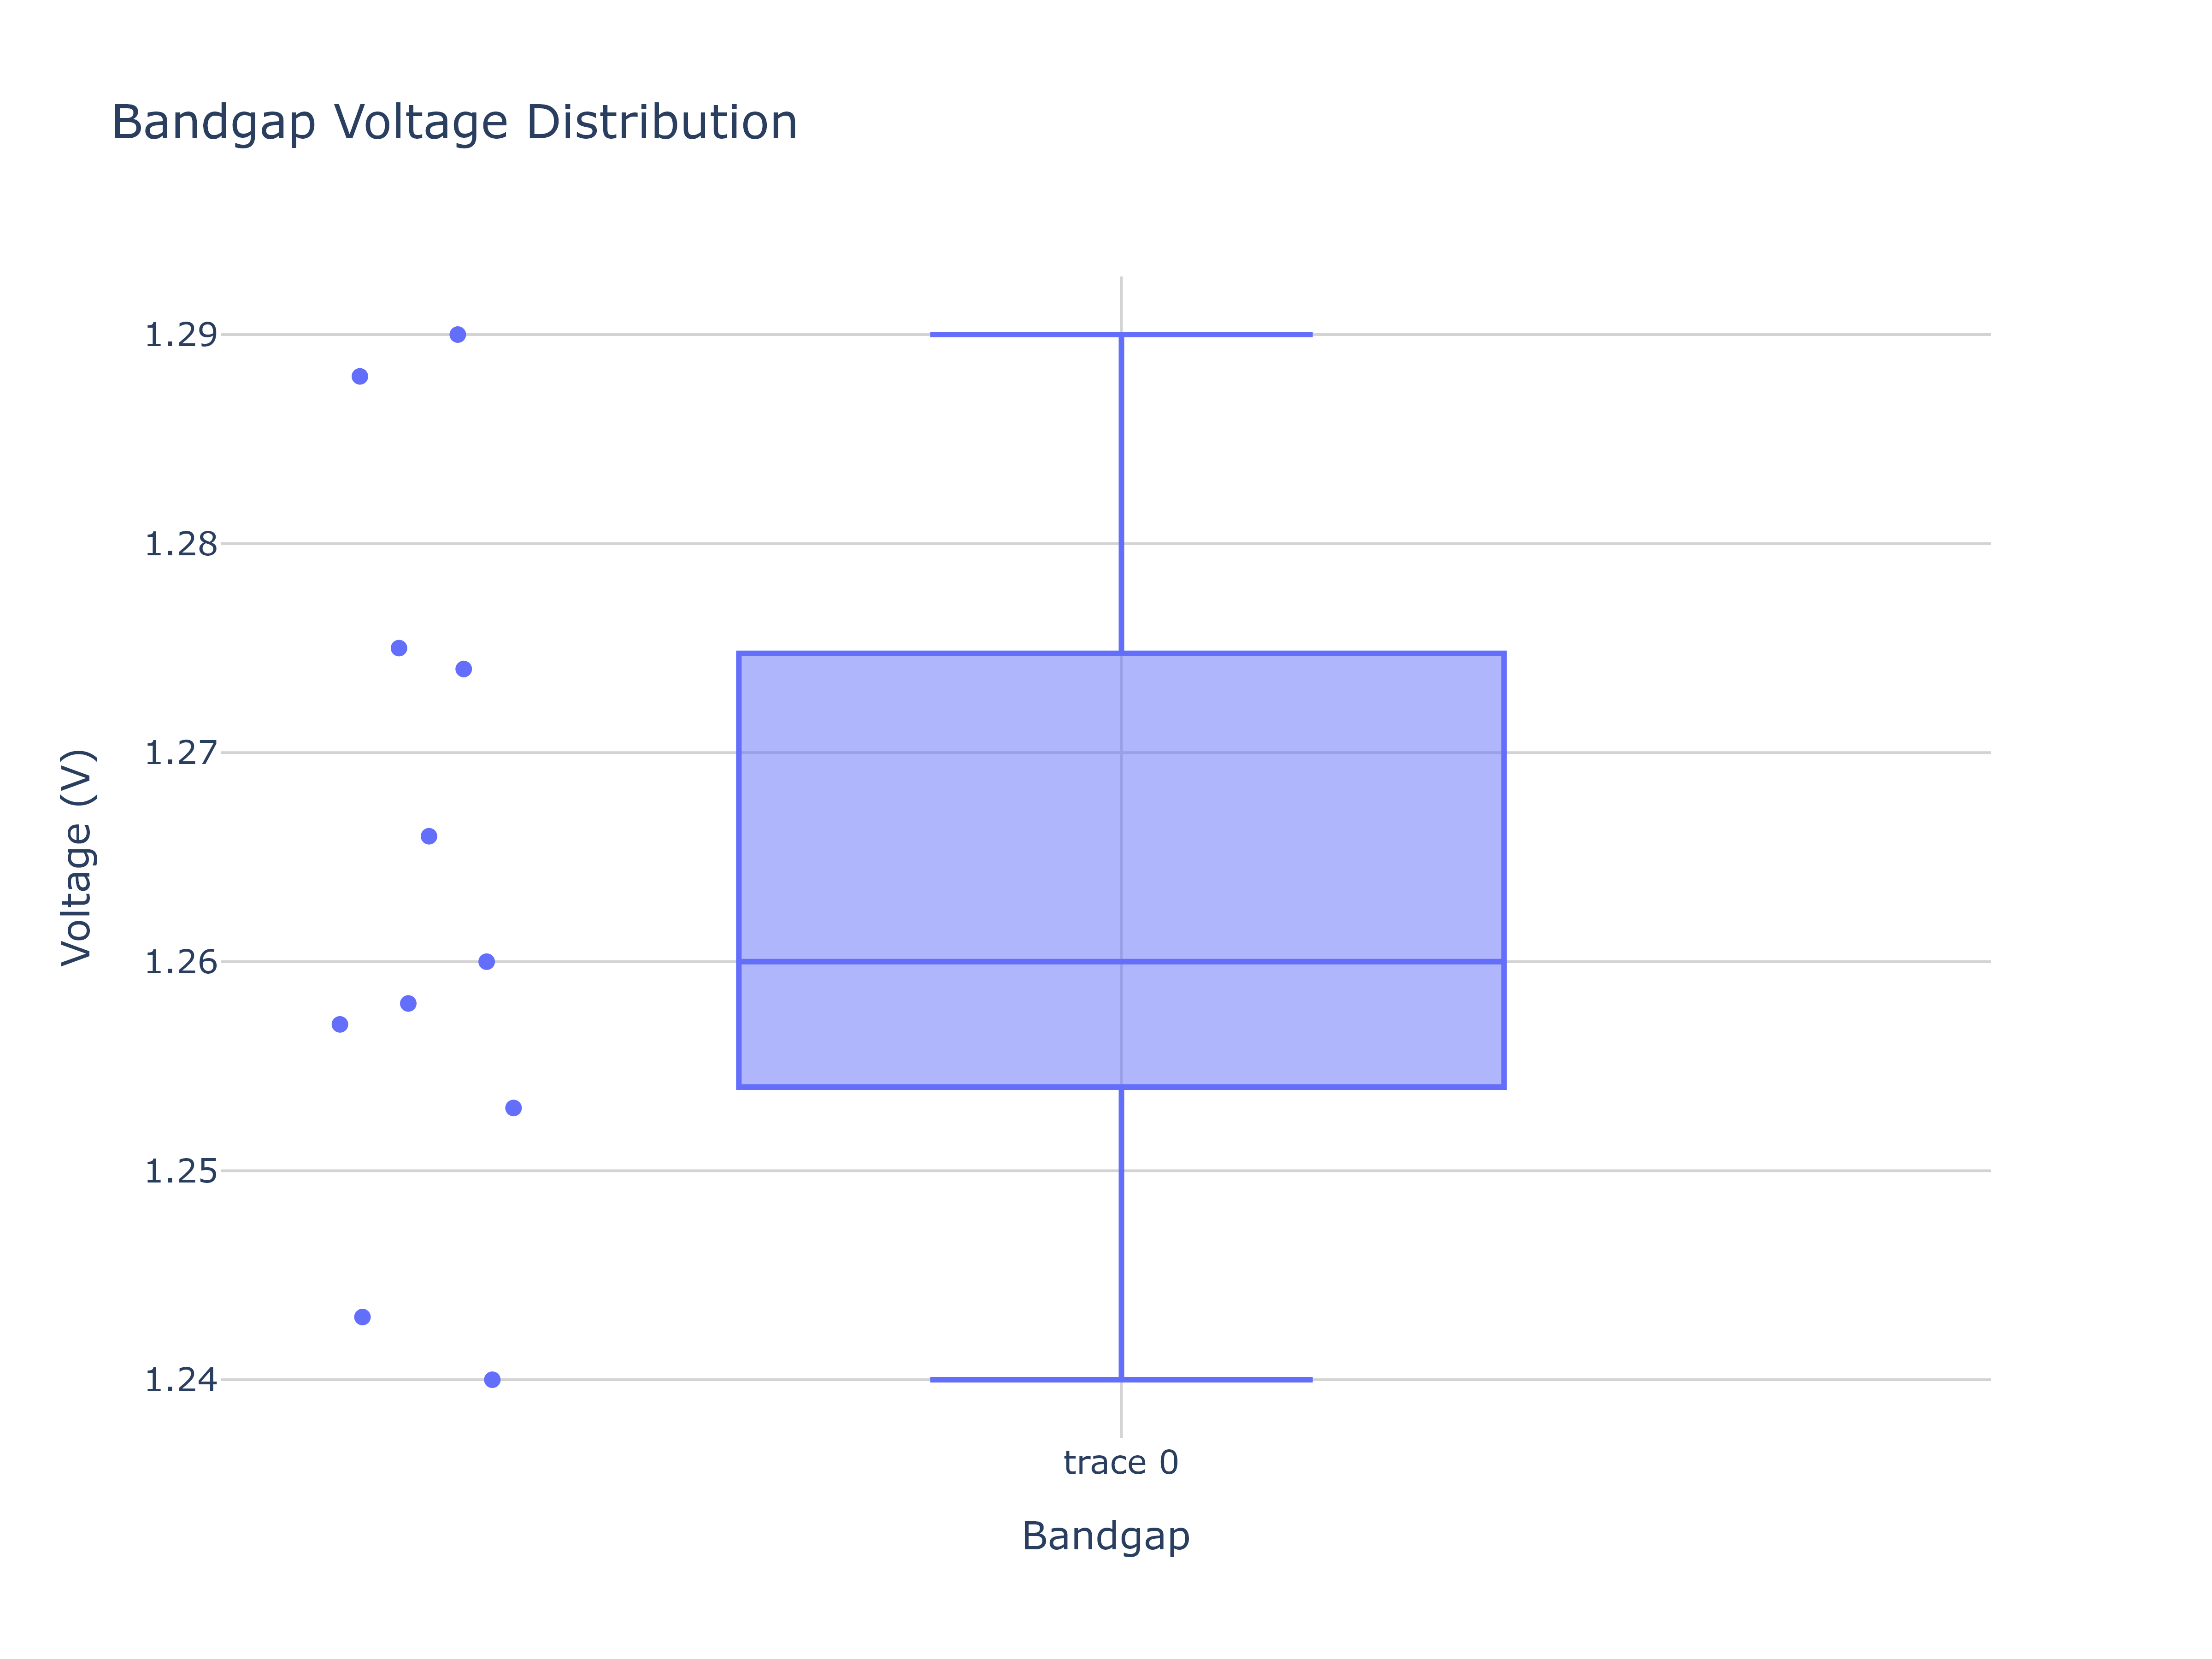
\includegraphics[width=\textwidth]{images/Bandgap_Voltage_Distribution.png}
	\caption{Bandgap voltage distribution at \qty{22}{\degreeCelsius} and 5V}
	\label{fig:bandgap_voltage_distrb}
\end{figure}

\begin{figure}[ht]
	\centering
	\includegraphics[width=\textwidth]{images/05_bandgap/band_volt_mc.pdf}
	\caption{Bandgap voltage Monte Carlo simulation (param.scs=3s, xh035.scs=mcg)}
	\label{fig:bandgap_voltage_mc}
\end{figure}
\clearpage
\subsection{Current Source}
\label{subsubsec:current_source}
The current source characteristics from the simulation can be seen in \autoref{tab:current_source} and \autoref{fig:ref_cur_mont}. The measurements have thereby shown that the current source is not in the range of of the simulation. The current measured is about \qty{4}{\micro\ampere} higher than the one simulated which corresponds to a derivation of $\left|\frac{\qty{14.3}{\micro\ampere}-\qty{10.3}{\micro\ampere}}{\qty{10.3}{\micro\ampere}}\right|\cdot 100\approx 38.8 \%$. An exact explanation for this behavior was not found, but since the oscillator has the same deviation and is independently of the current source the deviation most probably comes from the \glqq rmp1\grqq resistors since those were used in the layout of the oscillator and the current reference.
The current measured can be seen in \autoref{fig:current_source_distr}. About the other parameters no measurements could be done since the current source is not directly accessible.
\begin{longtable}{|p{3.5cm}|p{3.5cm}|p{3.5cm}|p{3.5cm}|}
	\hline
	\rowcolor{lightgray}
	\textbf{Description} &\textbf{Min} &\textbf{Max} & \textbf{Unit} \\ \hline
	
	Reference current & 8.4 & 13.5 &\qty{}{\micro\ampere} \\ \hline
	Current consumption & 50 & 81 & \qty{}{\micro\ampere} \\ \hline
	Min voltage (voltage where the trans resistance ($\frac{\Delta V_{in}}{\Delta I_{out}}$) is higher than \qty{1}{\mega\ohm}) & 3& 3.33 & \qty{}{\volt} \\ \hline
	\caption{Current reference characteristics} % needs to go inside longtable environment
	\label{tab:current_source}
\end{longtable}
\begin{figure}[ht]
	\centering
	\resizebox{1\textwidth}{!}{\includegraphics{images/06_current_ref/ref_cur_mont.pdf}}
	\caption{Monte Carlo distribution of Current reference. X-axis shows current through \glqq IPRB0\grqq{} in \autoref{fig:ref_cur_sim_schem} (param.scs=3s, xh035.scs=mcg)}
	\label{fig:ref_cur_mont}
\end{figure}
\begin{figure}[ht]
	\centering
	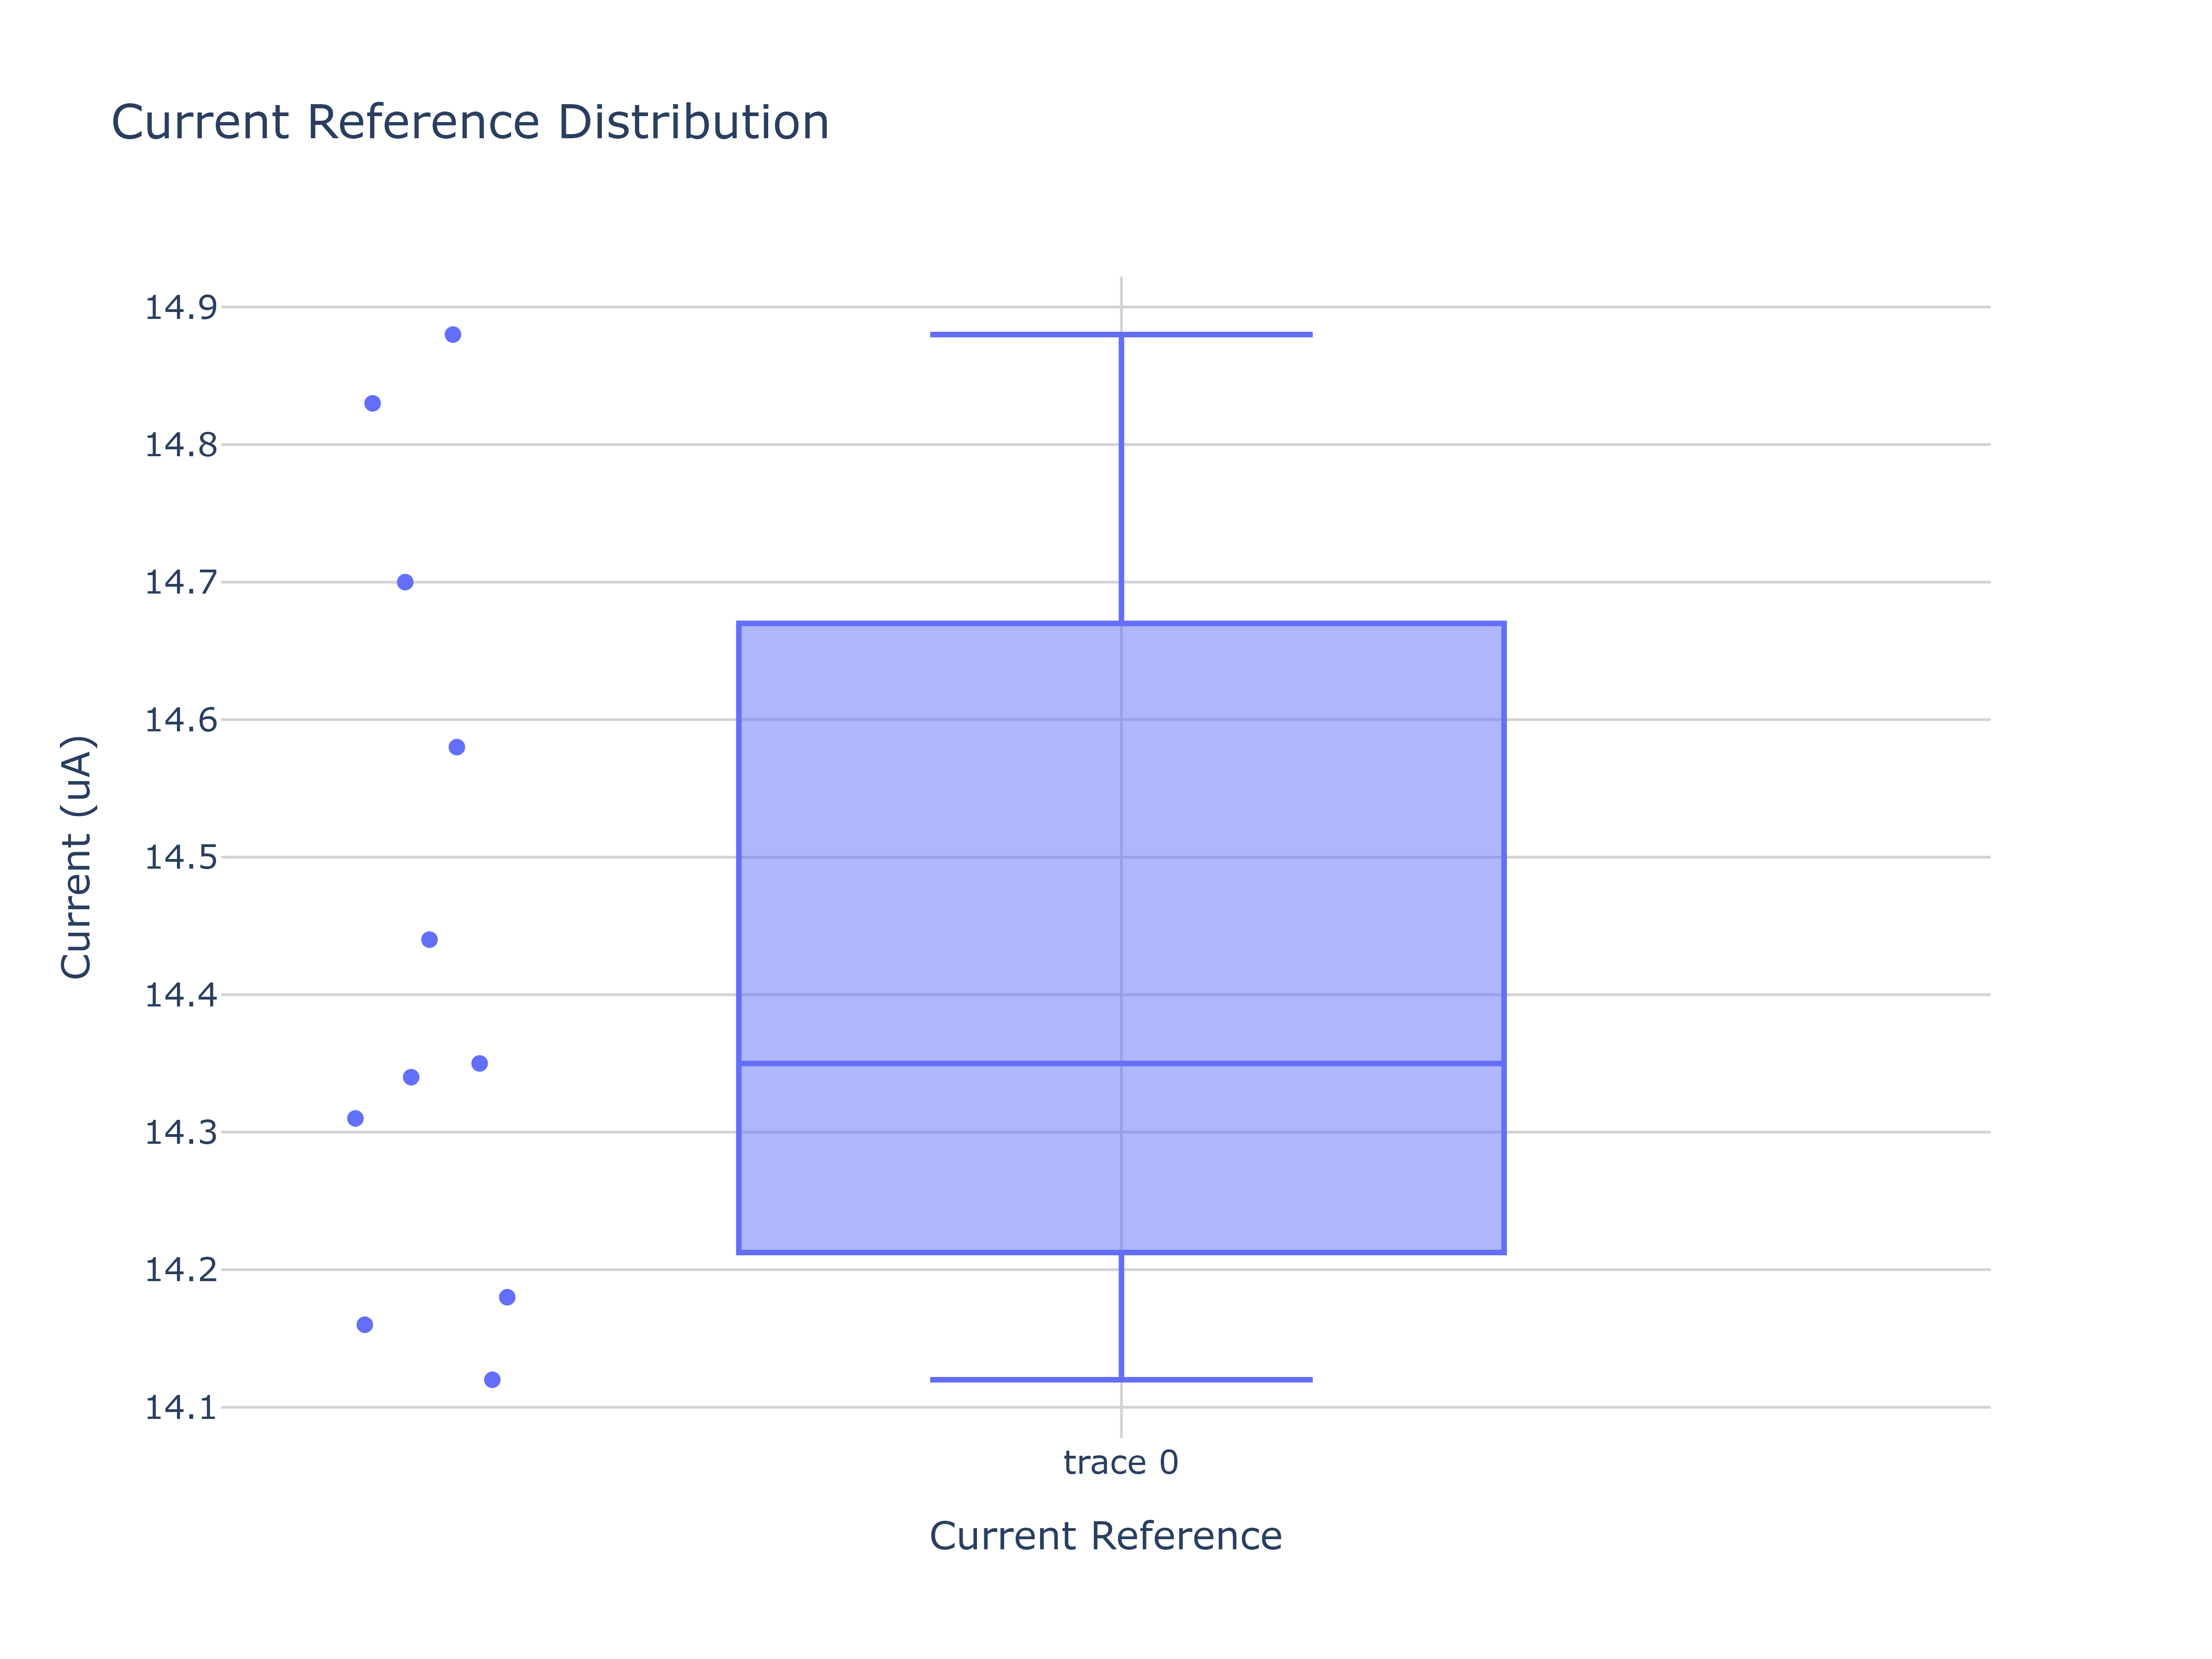
\includegraphics[width=\textwidth]{images/Current_Reference_Distribution.png}
	\caption{Current source distribution at \qty{22}{\degreeCelsius} and 5V}
	\label{fig:current_source_distr}
\end{figure}
\clearpage
\subsection{Oscillator}
\label{subsubsec:oscillator}
The oscillator characteristics from the simulation can be seen in \autoref{tab:osc}. The measurements have thereby shown that the oscillator is not in the range of of the simulation, when there is no configuration made over the SPI one has a nominal frequency of \qty{2.63}{\mega\hertz}, whereas in the simulation one had \qty{1.7}{\mega\hertz}, which results in an deviation of $\left|\frac{\qty{2.63}{\mega\hertz}-\qty{1.7}{\mega\hertz}}{\qty{1.7}{\mega\hertz}}\right|\cdot 100\approx 54.7 \%$, which is even more than in the current reference circuit. About the other parameters no measurements could be done since the oscillator is not directly accessible. Furthermore the frequency can also be tuned in the range of \qty{1.17}{\mega\hertz} to \qty{2.63}{\mega\hertz} over the spi registers (measured values) which results in the frequencies which can be seen in \autoref{tab:freq}. 
\begin{longtable}{|p{3.5cm}|p{3.5cm}|p{3.5cm}|p{3.5cm}|}
	\hline
	\rowcolor{lightgray}
	\textbf{Description} &\textbf{Min} &\textbf{Max} & \textbf{Unit} \\ \hline
	
	Frequency & 1.15 & 1.8 &\qty{}{\mega\hertz} \\ \hline
	Current consumption & 35 & 50 & \qty{}{\micro\ampere} \\ \hline
	Min voltage & 2& 3.187 & \qty{}{\volt} \\ \hline
	\caption{Specification} % needs to go inside longtable environment
	\label{tab:osc}
\end{longtable}
\begin{table}[h]
	\centering
	\begin{tabular}{|c|c|}
		\hline
		\rowcolor{lightgray}
		Register configuration & Frequency (MHz) \\
		\hline
		0 & \qty{2.63}{\mega\hertz} \\
		\hline
		1 & \qty{2.3}{\mega\hertz} \\
		\hline
		2 & \qty{2.19}{\mega\hertz} \\
		\hline
		3 & \qty{1.85}{\mega\hertz} \\
		\hline
		4 & \qty{1.67}{\mega\hertz} \\
		\hline
		5 & \qty{1.43}{\mega\hertz} \\
		\hline
		6 & \qty{1.27}{\mega\hertz} \\
		\hline
		7 & \qty{1.17}{\mega\hertz} \\
		\hline
	\end{tabular}
	\caption{Measured Frequencies with different configurations at \qty{22}{\degreeCelsius} and 5V}
	\label{tab:freq}
\end{table}


\clearpage


\subsection{Buck-Boost Converter}

\subsubsection{Start-up}
\label{sec:startup}
The start-up behavior shows significant differences to the results observed in simulations. Instead of the expected gradual increase in the output voltage, we observed the output voltage increase in distinct steps as can be seen in \autoref{fig:startup}. These distinct steps stem from the fact the input voltage collapses cyclicly to under the limit given by the \ac{POR}. The cycle can be described as the chip starting up and increasing the input current until the input voltage drops to bellow the limit given by the \ac{POR} thus disabling the chip and causing the input voltage to rise until the chip starts up again. The cycle continues until the output voltage reaches close to the nominal level and the outer voltage control loop regulates the current.  
The underlying issue is a misconfiguration of the internal registers causing the current limit to be disabled on start-up and the converter increasing the inductor current $I_L$ to unsustainable levels leading to the collapse of the input voltage. The cause is further described in \autoref{sec:missingcurrentlimit}.

\begin{figure}[ht]
	\centering
	
	\resizebox{1\textwidth}{!}{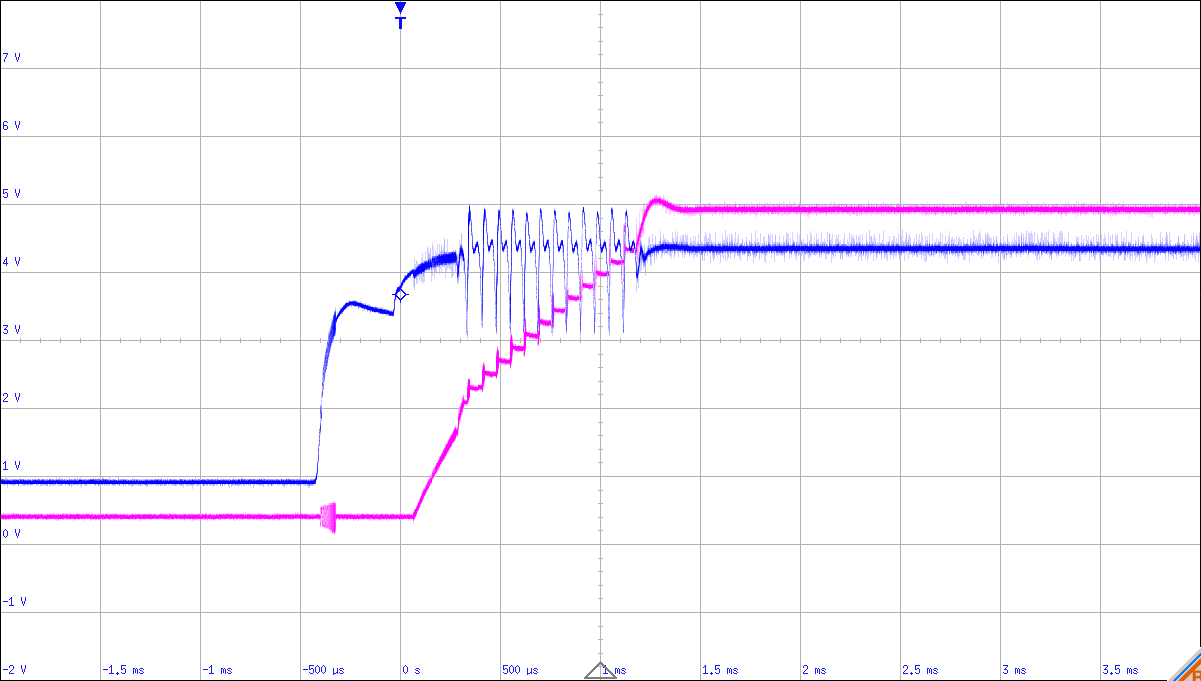
\includegraphics{images/07_DCDC/StartUp.PNG}}
	\caption{Start-up behavior without an attached load. Dark Blue: $V_{IN}$ measured; Pink: $V_{OUT}$ measured}
	\label{fig:startup}
\end{figure}


\subsubsection{Load Step Response}
The response to a load step is satisfactory and can be seen \autoref{fig:loadstep}. The regulation behavior is similar to the simulated response, but the measured controller has a higher bandwidth as can be seen in the faster response and is slightly overcompensated as it lacks the single oscillatory peak seen in the simulated response. Based on this response we estimate the implemented system has the following characteristics:

\begin{table}[H]
    \centering
    \begin{tabular}{|c|c|c|}
        Characteristic & Measured System & Simulation \\
        \hline
         Phase Margin  & \qty{55}{\degree} & \qty{45}{\degree}\\
		 Crossover Frequency & \qty{30}{\kilo\hertz} & \qty{20}{\kilo\hertz}  \\
    \end{tabular}
    \caption{Estimated regulator characteristics based on the response to a 200 mA load step}
    \label{tab:regChar}
\end{table}

\begin{figure}[ht]
	\centering
	
	\resizebox{1\textwidth}{!}{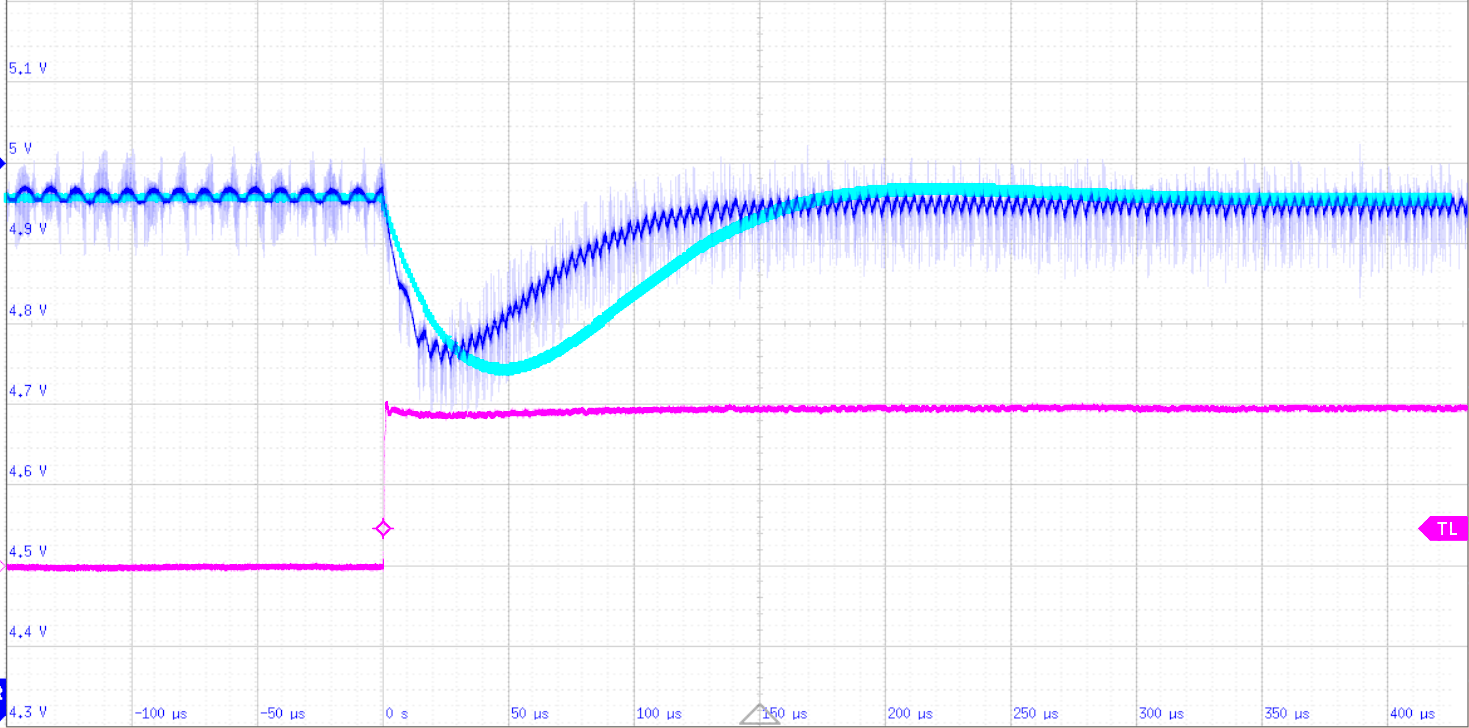
\includegraphics{images/07_DCDC/LoadStepVergleich.png}}
	\caption{Load regulation to a 200 mA load step for comparison between measured response and simulated response. Simulated response offset to remove constant load regulation error. Dark Blue: $V_{OUT}$ measured; Light Blue: $V_{OUT}$ simulated; Pink: $I_{OUT}$ measured}
	\label{fig:loadstep}
\end{figure}
\clearpage

\subsubsection{Load Regulation}
\label{sec:loadRegulation}
\begin{figure}[ht]
	\centering
	\resizebox{0.8\textwidth}{!}{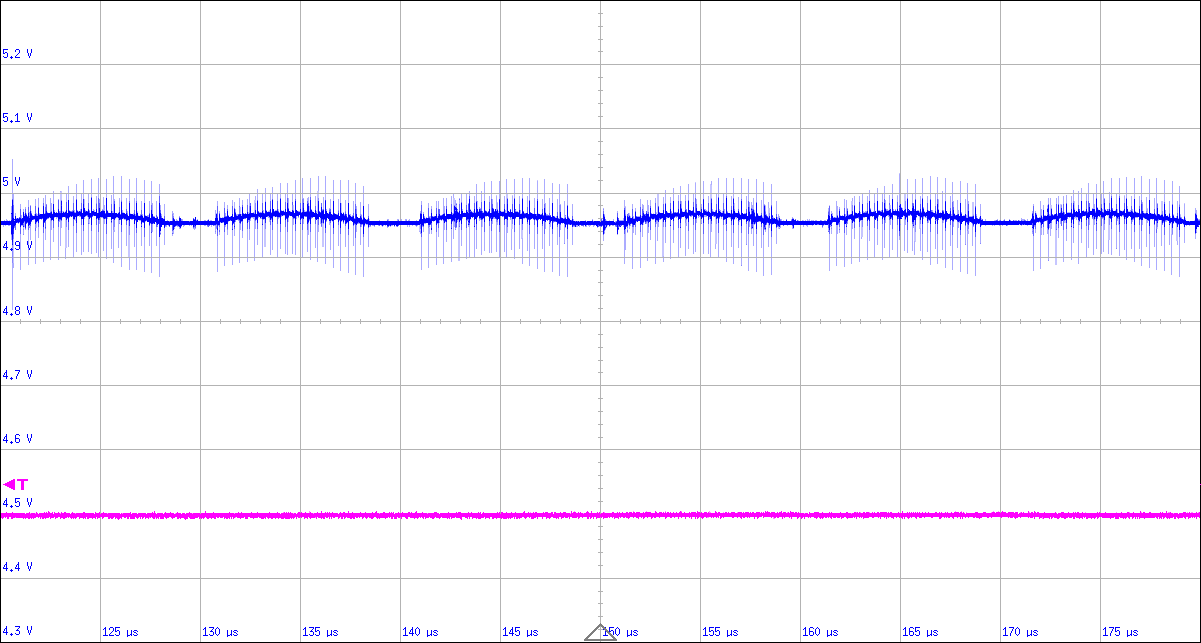
\includegraphics{images/07_DCDC/LoadSteadyState0mA.png}}
	\caption{Steady state load regulation with a 0mA load. Dark Blue: $V_{OUT}$; Pink: $I_{OUT}$}
\end{figure}
\begin{figure}[ht]
	\centering
	\resizebox{0.8\textwidth}{!}{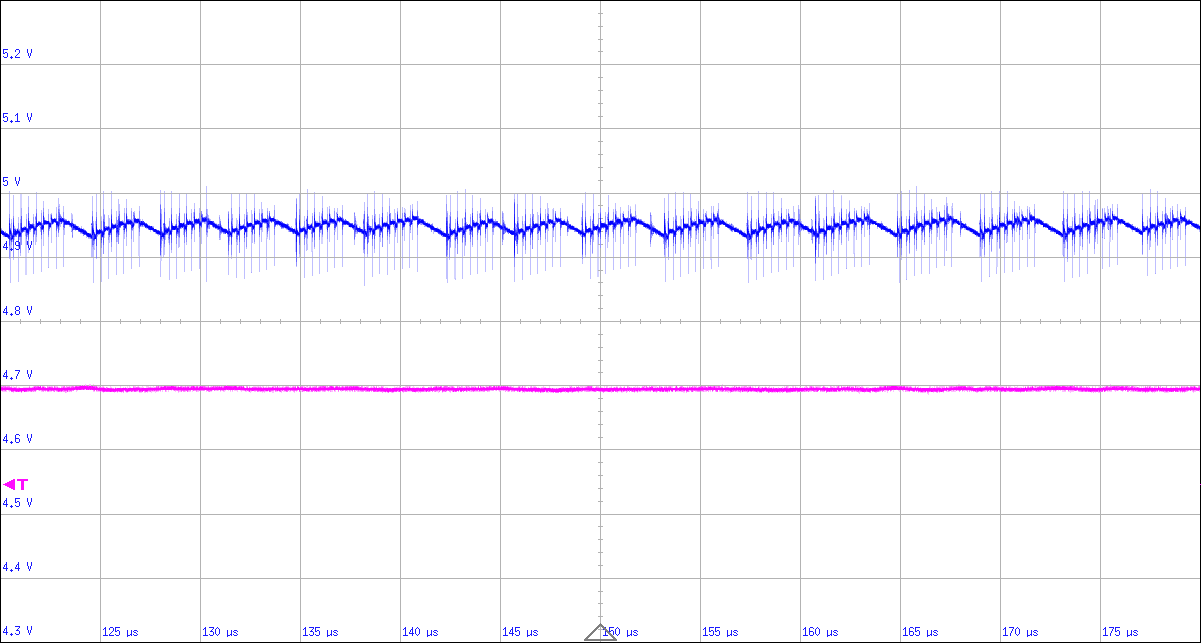
\includegraphics{images/07_DCDC/LoadSteadyState200mA.png}}
	\caption{Steady state load regulation with a 200mA load. Dark Blue: $V_{OUT}$; Pink: $I_{OUT}$}
\end{figure}
\clearpage



\foreach \i in {../ASIC-DESIGN-2/images/03_plots/DCDC Reset Test with 4.3V and resistor R2\, 70°C} {
    \begin{figure}[h]
        \centering
    \includegraphics[width=0.95\textwidth]{\i.pdf}
    %     \caption{\i}
    \end{figure}
    
}
\subsubsection{Efficiency}
\label{sec:efficiency}
%The efficiency of the TI chip was measured at different input voltages and loads. The efficiency was thereby callculated by difiding the output power by the input power. The results can be seen in \autoref{fig:efficiency TI chip}.
%\begin{figure}[h]
%    \centering
%    \includegraphics[width=0.8\textwidth]{../ASIC-DESIGN-2/images/03_plots/efficiencyTI.pdf}
%    \caption{Efficiency TI CHIP}
%    \label{fig:efficiency TI chip}
%\end{figure}

The conversion efficiency of our chip was measured under various load conditions and input voltage settings and can be seen in \autoref{fig:efficiency}. The measured values closely match our simulated values of \qty{83.5}{\percent} at \qty{200}{\milli\ampere} load current irrespective of the input voltage. The slight decrease in efficiency in comparison to the simulated values can be attributed to several not modeled influences such as bond wire resistance, losses in the input and output capacitors as well as losses else where outside of the chip. Of note is that the efficiency figures for \qty{20}{\milli\ampere} and \qty{50}{\milli\ampere} loads in \autoref{fig:efficiency} were estimated by linearly interpolating the measured input power levels at \qty{1}{\milli\ampere} and \qty{100}{\milli\ampere} and then dividing the known output power level by the calculated input power estimate.
\begin{figure}[h]
    \centering
    \begin{tikzpicture}
\begin{axis}[
    title={Efficiency versus Output Current},
    xlabel={Output Current [\qty{}{\milli\ampere}]},
    ylabel={Efficiency [\qty{}{\percent}]},
    xmin=0, xmax=300,
    ymin=0, ymax=100,
    xtick={0,100, 200, 300},
    ytick={0,20,40,60,80,100},
    legend pos=south east,
    ymajorgrids=true,
    grid style=dashed,
]

\addplot[
    color=blue,
    mark=square,
    ]
    coordinates {
    (1,4.5)(20,50)(50,70)(100,80)(200,78)(300,75.2)
    };
    \addlegendentry{$V_{IN} = \qty{5}{\volt}$}
     
\addplot[
    color=orange,
    mark=triangle,
    ]
    coordinates {
    (1,5.8)(20,46)(50,67)(100,78)(200,77)(300,71.5)
    };
    \addlegendentry{$V_{IN} = \qty{4.3}{\volt}$}
\addplot[
    color=mygreen,
    mark=o,
    ]
    coordinates {
    (1,3.7)(20,53)(50,71)(100,78)(200,79.8)(300,77.3)
    };
    \addlegendentry{$V_{IN} = \qty{5.5}{\volt}$}
      
\end{axis}
\end{tikzpicture}
    \caption{Conversion efficiency of our chip; Data points for 20 mA and 50 mA are estimates based on interpolation}
    \label{fig:efficiency}
\end{figure}
\clearpage
\subsubsection{Conversion Losses}
\label{sec:losses}
The total conversion losses can be put into two broad categories of switching frequency dependent switching losses and load dependent conduction losses shown in \autoref{eq:PLoss}. Our measured conversion losses can be seen in \autoref{fig:losses} and shows a roughly \qty{100}{\milli\watt} load independent loss, which explains the poor efficiency at sub \qty{100}{\milli\ampere} output currents seen in \autoref{fig:efficiency}. As output currents increase, the proportion of power lost due to switching decreases, leading to the improved efficiency at 100 to \qty{200}{\milli\ampere} range. With large output currents >\qty{200}{\milli\ampere} the conduction losses take over as they are proportional to the square of the output current leading again to a decrease in efficiency.

\begin{equation}
    P_{TOT} \approx P_{SWITCH} + P_{COND}
\end{equation}
\label{eq:PLoss}
with
\begin{equation*}
   P_{SWITCH} \propto 1
\end{equation*}
and 
\begin{equation*}
	P_{COND} \propto I_{OUT}^2
\end{equation*}

\begin{figure}[h]
    \centering
    \begin{tikzpicture}
\begin{axis}[
    title={Conversion Loss versus Output Current},
    xlabel={Output Current [\qty{}{\milli\ampere}]},
    ylabel={Power Loss [\qty{}{\milli\watt}]},
    xmin=0, xmax=300,
    ymin=0, ymax=600,
    xtick={0,100, 200, 300},
    ytick={0,100,200,300,400,500, 600},
    legend pos=north west,
    ymajorgrids=true,
    grid style=dashed,
]

\addplot[
    color=blue,
    mark=square,
    ]
    coordinates {
    (1,90.7)(100,124)(200,280)(300,485)
    };
    \addlegendentry{$V_{IN} = \qty{5}{\volt}$}
     
\addplot[
    color=orange,
    mark=triangle,
    ]
    coordinates {
    (1,68.8)(100,139.1)(200,290.5)(300,585.5)
    };
    \addlegendentry{$V_{IN} = \qty{4.3}{\volt}$}
\addplot[
    color=mygreen,
    mark=o,
    ]
    coordinates {
    (1,105.9)(100,139)(200,249.5)(300,434)
    };
    \addlegendentry{$V_{IN} = \qty{5.5}{\volt}$}
%\addplot[
%    color=purple,
%    mark=x,
%    ]
%    coordinates {
%    (1,100)(100,144)(200,276)(300,496)
%    };
%    \addlegendentry{$\qty{0.1}{\watt}+(\frac{1}{\qty{50}{\percent}}*I_{OUT})^2*\qty{1.1}{\ohm}$}
    
\end{axis}
\end{tikzpicture}

    \caption{Conversion losses at 1.17 MHz switching frequency}
    \label{fig:losses}
\end{figure}

\subsection{Device Characteristics}
\label{sec:characteristics}

	
	\section{Goal}



\subsection{abc}
	
	%%\section{Design}
%\label{chap:design}
%Upon completion of the literature research, a comprehensive understanding of the required components and their functionalities was gained. Utilizing a top-down approach, the design of the \ac{ASIC} commenced, wherein the different functionalities were divided into distinct blocks, as depicted in \autoref{fig:overview}. Initially, these blocks were implemented at a high abstraction level, and subsequently, in greater detail at the semiconductor level. This chapter provides an overview and description of each individual block, shedding light on their specific roles and characteristics.
%%After the literature research was completed it was mostly known which components are needed and how they work. Due to that the design of the \ac{ASIC} was started in a top down approach which means the different functionalities were divided into different blocks as one can see in \autoref{fig:overview}. The blocks itself were firstly implemented in a high abstraction design and afterwards in more detail on semiconductor level. An overview and description of the different blocks can therefore be found in this chapter.
%\begin{figure}[ht]
%	\centering
%	\includegraphics[width = \linewidth]{images/Overview2.drawio.pdf}
%	\caption{Our implementation of cascaded Buck Boost converter with active switches instead of diodes}
%	\label{fig:overview}
%\end{figure}
%
%\subsection{Input}
%The input block includes a POR circuit which makes sure that the circuit turns only on when the input voltage reaches a certain level, a Current reference which provides a input voltage and more or less temperature independent current source, a Band Gap reference which provides a input voltage and temperature independent voltage reference, a oscillator which provides a clock for the FSM.
%\subsubsection{Current source}
%Having a power supply (input voltage) independent current source is one of the key functionality for this project. Due to the fact that current sources are needed for multiple amplifier circuits which are included in function blocks such as the bandgap reference. \newline
%Since this problem was solved already multiple times before it was decided to go with a pre-existing solution/schematic. Lars Kamm therefore provided us with such a circuit, which was afterwards slightly adapted and will be discussed in this section. 
%%\paragraph{Bootstrap definition} 
%%According to \cite{Oxford_dict:bootstrap} bootstrap means: 'To make use of existing resources or capabilities to raise (oneself) to a new situation or state; to modify or improve by making use of what is already present. More recently, as transferred use of sense'\newline
%%For the bootstrap current source this means one creates a current source that is independent of the supply voltage, therefore it's name 'Bootstrap current source'. Note that the term 'Bootstrapping' is used for many completely different circuits as it can be seen in \cite{analog_design_essentials} (p.110).
%\paragraph{Circuit}
%At first glance comprehending a circuit like the one depicted in \autoref{fig:bootstrap4} may present some difficulties. Therefore, the following section provides a step-by-step description of the circuit.
%
%The concept behind the current reference circuit is to leverage the threshold voltage ($V_T$) of the MOSFET, as this parameter remains unaffected by the supply voltage, as indicated in \autoref{eq:mosfet_vt}. To fully comprehend the circuit in \autoref{fig:bootstrap4}, it is essential to grasp basic circuits such as the one shown in \autoref{fig:bootstrap1}. In this particular circuit, the voltage at the gate of $M_0$ is zero, resulting in the absence of a voltage $V_T$ anywhere. In order to establish the desired voltage $V_T$ across the transistor, a certain current $i_D$ must flow. Achieving this can be accomplished by introducing a current mirror into the circuit.
%\begin{figure}[ht]
%	\centering
%	\resizebox{0.3\textwidth}{!}{\subimport{./images/}{bootstrap1.tex}}
%	\caption{Current reference intro}
%	\label{fig:bootstrap1}
%\end{figure}
%When doing that one ends up with \autoref{fig:bootstrap2}. In \autoref{fig:bootstrap2} one has on the gate of $M_0$ the voltage $\Delta V_{GS}+V_T$ whereby $\Delta V_{GS}=V_{GS}-V_T$. When one now increases the ratio of $\frac{W}{L}$   $\Delta V_{GS}$ decreases as one can see from \autoref{eq:mos_ID}, which says: $\Delta V_{GS}=\sqrt{\frac{I_0}{\frac{\mu \cdot C_{ox}}{2} \frac{W}{L}}}$. Therefore when the ratio $\frac{W}{L}$ goes to infinity one would have a stable current through $R$ and a stable voltage on the gate of $M_0$, when one does not consider that $V_T$ is dependent on the temperature and the process. But the issue with the circuit in \autoref{fig:bootstrap2} is that one has a positive feedback loop, which means when the gate voltage on $M_0$ increases the current on $M_1$ and $M_2$ increases too, which increases the gate voltage of $M_0$ even more ($\Rightarrow$ Circuit is unstable). To prevent that one would need to insert an additional mosfet below $M_2$. But as one can see from this circuit one is still dependent on $V_{GS}$ when the ratio of $\frac{W}{L}$ is not infinity. 
%\begin{figure}[ht]
%	\centering
%	\resizebox{0.3\textwidth}{!}{\subimport{./images/}{bootstrap2.tex}}
%	\caption{Current reference example one }
%	\label{fig:bootstrap2}
%\end{figure}
%Let's therefore see if it gets better when one makes sure that the voltage is the same on the gate and the drain of $M_0$. One achieves this with the circuit in \autoref{fig:bootstrap3}. The gate voltage of $M_0$ is $\Delta V_{GS}+V_T$ and on $M_3$ and $M_4$ $2\cdot\Delta V_{GS}+2 \cdot V_T$. Therefore the voltage over R is $\Delta V_{GS}+V_T$. But when one decreases the ratio of $\frac{W}{L}$ of $M_4$ by a factor of 4 the voltage over R reduces to $V_T$ which means one gets rid of $\Delta V_{GS}$ and should therefore be completely independent of $V_{DD}$ \cite{youtube:bias}.
%\begin{figure}[ht]
%	\centering
%	\resizebox{0.3\textwidth}{!}{\subimport{./images/}{bootstrap3.tex}}
%	\caption{Current reference example two}
%	\label{fig:bootstrap3}
%\end{figure}
%\begin{figure}[ht]
%	\centering
%	\resizebox{0.3\textwidth}{!}{\subimport{./images/}{bootstrap4.tex}}
%	\caption{Current reference}
%	\label{fig:bootstrap4}
%\end{figure}
%When one tries to control the temperature dependency too one could add an additional nmos ($M_5$) above R with a $\frac{W}{L}$ x times larger than the one from $M_0$, as it can be seen in \autoref{fig:bootstrap4}. Since one knows that the voltage and the current on the source of $M_3$ and $M_4$ is the same one can write the following equations:
%$$
%\begin{aligned}
%	I_R=\frac{U_R}{R}\\
%	I_{S_{M_0}}=I_{S_{M_5}}\\
%	\sqrt{\frac{I_{S_{M_0}}}{\frac{\mu \cdot C_{ox}}{2}\frac{W}{L}\textcolor{gray}{\left(1+\lambda V_{DS}\right)}}}+V_T=\sqrt{\frac{I_{S_{M_5}}}{\frac{\mu \cdot C_{ox}}{2}\frac{W}{L}\textcolor{gray}{\left(1+\lambda V_{DS}\right)}\cdot x}}+V_T+U_r
%\end{aligned}
%$$
%The result of this equation is then (when one neglects the trivial solution where $I_{S_{M_0}}=I_{S_{M_5}}=0$ and the channel length modulation):
%$$
%I_{S_{M_0}}=I_{S_{M_5}}=\frac{2 \cdot \left(x\pm2\sqrt{x}+1\right) }{\beta\cdot\frac{W}{L}\cdot R^2 \cdot x} \text{ \textcolor{blue}{ !}}
%$$
%$$
%U_R=\frac{2 \cdot \left(x\pm2\sqrt{x}+1\right) }{\beta\cdot\frac{W}{L}\cdot R \cdot x} \text{ \textcolor{blue}{ !}}
%$$
%\textcolor{blue}{One solution from the equations above is an extraneous solutions.} The solutions that are really correct are: $I_{S_{M_0}}=I_{S_{M_5}}=\frac{2 \cdot \left(x-2\sqrt{x}+1\right) }{\beta\cdot\frac{W}{L}\cdot R^2 \cdot x}$ and $
%U_R=\frac{2 \cdot \left(x-2\sqrt{x}+1\right) }{\beta\cdot\frac{W}{L}\cdot R \cdot x}$.
%As one can see from those equations the current is depending on the factor of x and R one can therefore set it with setting x and R respectively. Furthermore it's worth to mention that R has a positive temperature coefficient and $V_{GS}$ a negative one. Therefore when the temperature increases the resistance $R$ gets higher while $V_{GS}$ gets lower. Due to that one could chose R and x in such a way that the circuit is more or less temperature independent. Due to the fact the amplifiers in the other circuits are also temperature dependent one chooses the ratio in such a way the the amplifiers are in the end not temperature dependent. But since this goes really deep into semiconductor physics no formulas for the temperature dependency of this circuits were derived. Nevertheless the simulation results were verified with the temperature independent equations which have shown that the calculations and simulations are quite similar.
%
%%$$
%%V_{\text {taw }}=\frac{k T}{q}=86.2 \frac{\mu V}{K} T
%%$$
%%One can now simplify the the equations to the following formula:
%%$$
%%\sqrt{\frac{I_{S_{M_0}}}{\frac{\mu \cdot C_{ox}}{2}\frac{W}{L}}}+V_T=\sqrt{\frac{I_{S_{M_0}}}{\frac{\mu \cdot C_{ox}}{2}\frac{W}{L}\cdot x}}+V_T+I_{S_{M_0}} \cdot R
%%$$
%%$$
%%\frac{I_{S_{M_0}}}{\frac{\mu \cdot C_{ox}}{2}\frac{W}{L}}=\frac{I_{S_{M_0}}}{\frac{\mu \cdot C_{ox}}{2}\frac{W}{L}\cdot x}+\sqrt{\frac{I_{S_{M_0}}}{\frac{\mu \cdot C_{ox}}{2}\frac{W}{L}\cdot x}} \cdot (I_{S_{M_0}} \cdot R)+\left(I_{S_{M_0}} \cdot R \right)^2
%%$$
%%
%%$$
%%a=\left(I_{S_{M_0}} \cdot R \right)^2
%%$$
%%
%%$$
%%b=\frac{I_{S_{M_0}} \cdot (1-x)}{\frac{\mu \cdot C_{ox}}{2}\frac{W}{L}}
%%$$
%%
%%$$
%%c=0
%%$$
%%$$
%%x_{1,2}=\frac{-b \pm \sqrt{b^2-4 a c}}{2 a}
%%$$
%%solve(((ur)/(r))=i00 and i00=i05 and √(((i00)/(((beta)/(2))*wl)))+vt=√(((i05)/(((beta)/(2))*wl*x)))+vt+ur,i00,i05,ur)
%When inserting the values of the circuit one gets the following result:
%
%$$
%I_{S_{M_0}}=I_{S_{M_5}}=\frac{2 \cdot \left(16-2\sqrt{16}+1\right) }{\SI[group-digits=true]{103e-6}{\ampere\per\volt\squared} \cdot16\cdot \SI[group-digits=true]{22.5e-3}{\ohm}^2 \cdot 16}=\SI[group-digits=true]{2.697e-6}{\ampere}
%$$
%$$
%U_R=\frac{2 \cdot \left(16-2\sqrt{16}+1\right) }{\SI[group-digits=true]{103e-6}{\ampere\per\volt\squared} \cdot16\cdot \SI[group-digits=true]{22.5e-3}{\ohm} \cdot 16}=\SI[group-digits=true]{168.554}{\milli\volt}
%$$
%with:
%\begin{description}
%	[font=\normalfont,leftmargin=1.9in,style=multiline]
%	\item[$\beta$]
%	$\qty{103}{\micro\ampere\per\volt\squared}$
%	\item[$R$]
%	\qty{22.5}{\kilo\ohm}
%	\item[$\frac{W}{L}$]
%	8
%	\item[$x$]
%	16
%\end{description}
%This similar to the simulation (simulation\footnote{Simulation result can be found in \autoref{fig:bootstrap_mon} in the appendix}: $\SI[group-digits=true]{4.9}{\micro\ampere}$, calculation: $\SI[group-digits=true]{2.7}{\micro\ampere}$).
%
%
%
%\begin{figure}[ht]
%	\centering
%	
%	\resizebox{1\textwidth}{!}{\includegraphics{../ASIC-DESIGN/data/03_Plots/02_Bootstrap/ref_cur_mont.pdf}}
%	\caption{Monte Carlo distribution of Current reference. X-axis shows current through \glqq IPRB0\grqq{} in \autoref{fig:ref_cur_sim_schem} (param.scs=3s, xh035.scs=mcg)}
%	\label{fig:ref_cur_mont}
%\end{figure}
%
%The implemented design on the chip can be seen in \autoref{fig:bootstrap5}. For simplicity one can neglect in a first step M89, M10, M13, M19 and M21. When doing that one sees in \autoref{fig:bootstrap5} the same circuit as in \autoref{fig:bootstrap4} with some additions (M51 and M52 are not needed they were introduced in the layout for a common centroid design). This additions are needed since one has two operating points as one saw before. To be in the right operating point a so called start up circuit is needed which will be explained in more detail. On the left of \autoref{fig:bootstrap5} one finds the enable signal EN and its inverted signal ENN. In turned off state M15 is conducting an therefore M14 discharged, furthermore VB4 is pulled to VDDA which forces the bootsrap to be in state zero (state where no current is flowing). When the circuit is turned on  M8, M9 and M11 are conducting, since their gate voltage is zero which leads to the fact that the node voltage of N2 is pulled to VDDA. Furthermore VB4 is not any more pulled to VDDA. The voltage in N2 causes a current in the Current reference which is mirrored to M5, which charges the capacitor M14 and finally stops N2 to be pulled to VDDA. The Current reference is now in its operating state where current is flowing. This current can then be further mirrored to other components with VB4, VB3, VB2 and VB1.
%\begin{figure}[ht]
%	\centering
%	\includegraphics[width=\textwidth]{../ASIC-DESIGN/data/03_Plots/02_Bootstrap/ref_cur_schem.png}
%	\caption{Current reference Implemented}
%	\label{fig:bootstrap5}
%\end{figure}
%\autoref{fig:ref_cur_sim_schem} shows the testbench used to test the current reference circuit. 
%\begin{figure}[ht]
%	\centering
%	\includegraphics[width=\textwidth]{../ASIC-DESIGN/data/03_Plots/02_Bootstrap/ref_cur_sim_schem.png}
%	\caption{Current reference test bench}
%	\label{fig:ref_cur_sim_schem}
%\end{figure}
%
%
%\autoref{fig:ref_cur_cur} shows the current in dependency of the supply voltage. 
%\begin{figure}[ht]
%	\centering
%	\includegraphics[width=\textwidth]{../ASIC-DESIGN/data/03_Plots/02_Bootstrap/ref_cur_cur.pdf}
%	\caption{Current reference current vs supply voltage}
%	\label{fig:ref_cur_cur}
%\end{figure}
%\autoref{fig:boot_out_res} shows the transresistance of the Input voltage to the output current. It is visible from this plot that the current reference should be operated with a voltage greater than 3.3V to have a input voltage independent current.
%\begin{figure}[ht]
%	\centering
%	\includegraphics[width=\textwidth]{../ASIC-DESIGN/data/03_Plots/02_Bootstrap/ref_cur_tran_res.pdf}
%	\caption{Current reference trans resistance $\frac{\Delta V_{in}}{\Delta I_{out}}$}
%	\label{fig:boot_out_res}
%\end{figure}
%
%\autoref{fig:boot_out_res_2} shows the output resistance of the current reference ($V_4$ in \autoref{fig:ref_cur_sim_schem}) divided by the current that goes into the source of $V_4$ at different voltages. This allows to estimate how many diode voltage one is allowed to use to mirror the reference current. It shows that the voltage of the diode must be at least one 0.8V below the supply voltage.
%\begin{figure}[ht]
%	\centering
%	\includegraphics[width=\textwidth]{../ASIC-DESIGN/data/03_Plots/02_Bootstrap/ref_cur_res.pdf}
%	\caption{Current reference output resistance $\frac{\Delta V_{out}}{\Delta I_{out}}$}
%	\label{fig:boot_out_res_2}
%\end{figure}
%%\begin{figure}[ht]
%%	\centering
%%	\includegraphics[width=\textwidth]{../ASIC-DESIGN/data/03_Plots/02_Bootstrap/09_bootstrap_tb_2.png}
%%	\caption{Current reference test bench two}
%%	\label{fig:bot_tb_schem2}
%%\end{figure}
%
%
%%\begin{figure}[ht]
%%	\centering
%%	\includegraphics[width=\textwidth]{../ASIC-DESIGN/data/03_Plots/02_Bootstrap/06_test_results.png}
%%	\caption{Current reference test}
%%	\label{fig:boot_test}
%%\end{figure}
%The summarized specification of the block can be found in \autoref{tab;bootstrap}.
%\begin{longtable}{|p{3.5cm}|p{3.5cm}|p{3.5cm}|p{3.5cm}|}
%	\hline
%	\rowcolor{lightgray}
%	\textbf{Description} &\textbf{Min}  &\textbf{Max} & \textbf{Unit} \\ \hline
%	
%	Reference current & 8.4 & 13.5 &\qty{}{\micro\ampere} \\ \hline
%	Current consumption & 50 & 81 & \qty{}{\micro\ampere} \\ \hline
%	Min voltage (voltage where the trans resistance ($\frac{\Delta V_{in}}{\Delta I_{out}}$) is higher than \qty{1}{\mega\ohm}) & 3& 3.33 & \qty{}{\volt} \\ \hline
%	\caption{Current reference characteristics} % needs to go inside longtable environment
%	\label{tab:booststrap}
%\end{longtable}
%
%\clearpage
%
%\subsubsection{Bandgap}
%For the \href{https://youtu.be/ncZzxvG4XOM}{Bandgap reference} a given implementation of a 3.3V circuit from X-Fab was taken and adapted for the 5V technology. The final design can be seen in \autoref{fig:bandgap_schem}.
%
%\begin{figure}[ht]
%	\centering
%	\includegraphics[width=\textwidth]{../ASIC-DESIGN/data/03_Plots/03_Bandgap/band_gap_schem.png}
%	\caption{Bandgap schematic}
%	\label{fig:bandgap_schem}
%\end{figure}
%
%For the test the schematic in \autoref{fig:bandgap_tb_schem} was used, where EN is set to 5V and ENN to 0V furthermore VddA was sweept from 0V to 5.5V
%\begin{figure}[ht]
%	\centering
%	\includegraphics[width=\textwidth]{../ASIC-DESIGN/data/03_Plots/03_Bandgap/band_gap__tb_schem.png}
%	\caption{Bandgap testbench}
%	\label{fig:bandgap_tb_schem}
%\end{figure}
%
%\autoref{fig:bandgap_voltage_vs_supplyv} shows that the bandgap voltage is quite stable over the corners, but  slight variations can be seen in \autoref{fig:bandgap_voltage_mc} the montecarlo simulation. Since the output voltage of the DC/DC converter is anyway exactly set by a external resistor only the variance over the temperature and supply voltage plays a major role. Which is very low as can be seen in \autoref{fig:bandgap_voltage_vs_supplyv} and \autoref{fig:bandgap_voltage_vs_temp}.
%\begin{figure}[ht]
%	\centering
%	\includegraphics[width=\textwidth]{../ASIC-DESIGN/data/03_Plots/03_Bandgap/band_volt_volt.pdf}
%	\caption{Bandgap voltage vs supplyvoltage}
%	\label{fig:bandgap_voltage_vs_supplyv}
%\end{figure}
%\begin{figure}[ht]
%	\centering
%	\includegraphics[width=\textwidth]{../ASIC-DESIGN/data/03_Plots/03_Bandgap/band_volt_mc.pdf}
%	\caption{Bandgap voltage Montecarlo simulation (param.scs=3s, xh035.scs=mcg)}
%	\label{fig:bandgap_voltage_mc}
%\end{figure}
%
%\begin{figure}[ht]
%	\centering
%	\includegraphics[width=\textwidth]{../ASIC-DESIGN/data/03_Plots/03_Bandgap/04_Test.png}
%	\caption{Bandgap test output}
%	\label{fig:bandgap_test}
%\end{figure}
%\autoref{fig:bandgap_voltage_vs_temp} shows the dependency of the bandgap voltage vs the temperature.
%\begin{figure}[ht]
%	\centering
%	\includegraphics[width=\textwidth]{../ASIC-DESIGN/data/03_Plots/03_Bandgap/band_volt.pdf}
%	\caption{Bandgap voltage vs temperature}
%	\label{fig:bandgap_voltage_vs_temp}
%\end{figure}
%
%\autoref{tab:bandgap} Show the characteristics of the bandgap design used in this project.
%\begin{longtable}{|p{3.5cm}|p{3.5cm}|p{3.5cm}|p{3.5cm}|}
%	\hline
%	\rowcolor{lightgray}
%	\textbf{Description} &\textbf{Min}  &\textbf{Max} & \textbf{Unit} \\ \hline
%	
%	Bandgap voltage & 1.226 & 1.277 &\qty{}{\volt} \\ \hline
%	Current consumption & 16.73 & 23.53 & \qty{}{\micro\ampere} \\ \hline
%	Min voltage & 2.3& 2.9 & \qty{}{\volt} \\ \hline
%	\caption{Bandgap characteristic} % needs to go inside longtable environment
%	\label{tab:bandgap}
%\end{longtable}
%\clearpage
%
%\subsubsection{Oscillator}
%For the digital part of the circuit there is a clock required to process the data received over the SPI. \footnote{It was decided to generate an internal clock although it would have been possible to build a finite state machine which uses the SPI signal only to read and write the registers.} Since the SPI standard does not define a certain clock speed the frequency generated in the \ac{ASIC} plays a minor role. Due to that it was decided to generate the clock with a sawtooth generator (a capacitor gets charged with a certain current and as soon as it reaches a threshold it gets discharged) due to the fact that this approach is very easy to implement and fully compatible with the CMOS process used.
%The design used can be seen in \autoref{fig:osc_schem}.
%\begin{figure}[ht]
%	\centering
%	\includegraphics[width=\textwidth]{../ASIC-DESIGN/data/03_Plots/04_Clock/01_Oscillator_schematic.png}
%	\caption{Oscillator schematic}
%	\label{fig:osc_schem}
%\end{figure}
%As the name tells it delivers a define current to the circuit, which is used to charge the capacitor M7. As soon as the voltage at the drain of M0 reaches a certain threshold the smith trigger triggers and discharges the cap over R0. Due to the fact that the cap gets much faster discharged than charged the signal after the smith trigger is only a short impulse. To get a clock with a duty cycle of about 50\% a d-flipflop was added which changes it's value by every impulse. This reduces the clock frequency by a factor of two but allows to achieve the previously mentioned duty cycle.
%
%The test bench used to validate the design can be seen in \autoref{osc_tb}.
%\begin{figure}[ht]
%	\centering
%	\includegraphics[width=\textwidth]{../ASIC-DESIGN/data/03_Plots/04_Clock/02_Oscillator_tb_schematic.png}
%	\caption{Oscillator test bench schematic}
%	\label{fig:osc_tb}
%\end{figure}
%The EN signal was set to 5V and the ENN to 0V whereas the VddA voltage was swept from 0V to 5V. From \autoref{fig:osc_freq_volt} one sees the circuit works from about 3.2V. 
%\begin{figure}[ht]
%	\centering
%	\includegraphics[width=\textwidth]{../ASIC-DESIGN/data/03_Plots/04_Clock/03_oscillator_frequency_vs_voltage_plot_compressed.pdf}
%	\caption{Oscillator frequency vs voltage}
%	\label{fig:osc_freq_volt}
%\end{figure}
%The exact value can be read from \autoref{fig:osc_test}, which says 3.187V.
%\begin{figure}[ht]
%	\centering
%	\includegraphics[width=\textwidth]{../ASIC-DESIGN/data/03_Plots/04_Clock/04_Test.png}
%	\caption{Oscillator test output}
%	\label{fig:osc_test}
%\end{figure}
%The most important Values can be read from \autoref{tab:osc} and further values can be read from \autoref{fig:osc_test}.
%\begin{longtable}{|p{3.5cm}|p{3.5cm}|p{3.5cm}|p{3.5cm}|}
%	\hline
%	\rowcolor{lightgray}
%	\textbf{Description} &\textbf{Min}  &\textbf{Max} & \textbf{Unit} \\ \hline
%	
%	Frequency & 1.15 & 1.7 &\qty{}{\mega\hertz} \\ \hline
%	Current consumption & 35 & 50 & \qty{}{\micro\ampere} \\ \hline
%	Min voltage & 2& 3.187 & \qty{}{\volt} \\ \hline
%	\caption{Specification} % needs to go inside longtable environment
%	\label{tab:osc}
%\end{longtable}
%
%\clearpage
%\subsubsection{POR}
%For the POR circuit an example was provided by Lars Kamm and afterwards adapted, so that it has the right power on voltage and delay time. The final design can be seen in \autoref{fig:por_schem}.
%
%\begin{figure}[ht]
%	\centering
%	\includegraphics[width=\textwidth]{../ASIC-DESIGN/data/03_Plots/01_POR/03_por_schem.png}
%	\caption{POR schematic}
%	\label{fig:por_schem}
%\end{figure}
%The test bench with which the design was tested is visible in \autoref{fig:por_tb_schem}
%\begin{figure}[ht]
%	\centering
%	\includegraphics[width=\textwidth]{../ASIC-DESIGN/data/03_Plots/01_POR/02_por_tb_schem.png}
%	\caption{POR testbench schematic}
%	\label{fig:por_tb_schem}
%\end{figure}
%In \autoref{fig:por_test} the test sequence for the delay measurement is visible. In yellow one sees the supply voltage and in red the PORB signal. Which is on high when the circuit should work.
%
%\begin{figure}[ht]
%	\centering
%	\includegraphics[width=\textwidth]{../ASIC-DESIGN/data/03_Plots/01_POR/04_por_tran2.pdf}
%	\caption{POR transient simulation}
%	\label{fig:por_tran}
%\end{figure}
%
%
%\autoref{fig:por_test} show the test output of the testbench. It's output is summarized in \autoref{tab:por}.
%\begin{figure}[ht]
%	\centering
%	\includegraphics[width=\textwidth]{../ASIC-DESIGN/data/03_Plots/01_POR/01_POR_test.png}
%	\caption{POR test output}
%	\label{fig:por_test}
%\end{figure}
%
%\begin{longtable}{|p{3.5cm}|p{3.5cm}|p{3.5cm}|p{3.5cm}|}
%	\hline
%	\rowcolor{lightgray}
%	\textbf{Description} &\textbf{Min}  &\textbf{Max} & \textbf{Unit} \\ \hline
%	
%	input delay & 26 & 44 &\qty{}{\micro\second} \\ \hline
%	output delay & 4.4 & 6.8 &\qty{}{\micro\second} \\ \hline
%	Current consumption & 13 & 31 & \qty{}{\micro\ampere} \\ \hline
%	Min voltage & 3.176& 3.7 & \qty{}{\volt} \\ \hline
%	\caption{POR characteristic} % needs to go inside longtable environment
%	\label{tab:por}
%\end{longtable}
%\clearpage
%
%
%
%\subsubsection{Top test bench}
%To check if the total circuit with all the components is working a global test bench was created, which uses a SPI signal generator. In \autoref{fig:spi1} one sees that the SPI generator tries to write to register one the value 0xAA, which is actually not allowed, since register one is read only. As one sees register one also does not get written.
%\begin{figure}[ht]
%	\centering
%	\includegraphics[width=\textwidth]{../ASIC-DESIGN/data/03_Plots/06_SPI/01_write_to_reg_1_not_possible.png}
%	\caption{SPI signal one}
%	\label{fig:spi1}
%\end{figure}
%For the next steps the content from register two was changed as it can be seen in \autoref{fig:spi2} and \autoref{fig:spi3}. Which is working as one would expect. The content on register two is used to mux a corresponding analog signal to the output.
%\begin{figure}[ht]
%	\centering
%	\includegraphics[width=\textwidth]{../ASIC-DESIGN/data/03_Plots/06_SPI/02_write_02_to_register_2.png}
%	\caption{SPI signal two}
%	\label{fig:spi2}
%\end{figure}
%\begin{figure}[ht]
%	\centering
%	\includegraphics[width=\textwidth]{../ASIC-DESIGN/data/03_Plots/06_SPI/03_write_03_to_register_2_miso_should_be_2.png}
%	\caption{SPI signal three}
%	\label{fig:spi3}
%\end{figure}
%\subsubsection{Conclusion Input blocks}
%As seen in the previous section, we have successfully designed, simulated, and tested all the input blocks. While a comprehensive explanation of the current reference circuit was provided, we have not delved into the same level of detail for the other blocks. This is because these blocks are less complex and are already well-documented in publicly available resources. Additionally, for the reader, the precise implementation and calculations may not be crucial. The simulation results hold greater significance since they utilize more accurate transistor models compared to our manual calculations. Nonetheless, manual analysis and understanding of the circuit's underlying concepts remain helpful in conjunction with the simulation results.
%
%
%
%\subsection{Pads}
%In order to achieve the required 200mA output, it became apparent that a single pad per input and output on the ASIC is insufficient to handle such high currents. According to the datasheet, each pad can handle up to 50mA. As a result, it was decided to utilize a chip with 48 pads, distributed evenly with 12 on each side. This arrangement allows that the Inductor, hearing instruments, GND and VDD pad have multiple pads.
%
%Referring to \autoref{tab:PADS}, it is evident that 39 pads are definitely necessary, and an additional 9 pads remain unassigned but could potentially be utilized in the layout phase to further decrease the input resistance of the high current connections.
%\begin{figure}[ht]
%	\centering
%	\includegraphics[width=0.5\textwidth]{images/pad_ring.png}
%	\caption{Pad ring}
%	\label{fig:pad_ring}
%\end{figure}
%\begin{figure}[htb]
%	\centering % <-- added
%	\begin{subfigure}{0.45\textwidth}
%		%[trim={left bottom right top},clip]
%		\includegraphics[page=335,clip, trim=0.5cm 18cm 0.5cm 6.5cm, width=1.00\textwidth]{data/01_X-Fab/02_xh035-UserGuide-IO_Library-v10_2_0.pdf}
%		\caption{APR00DF5 (\cite{xfab:io_library_manual} p.335)}
%		\label{fig:APR00DP5}
%	\end{subfigure}\hfil % <-- added
%	\begin{subfigure}{0.45\textwidth}
%		%[trim={left bottom right top},clip]
%		\includegraphics[page=350,clip, trim=0.5cm 19.5cm 0.5cm 6.5cm, width=1.00\textwidth]{data/01_X-Fab/02_xh035-UserGuide-IO_Library-v10_2_0.pdf}
%		\caption{VDDALLPADF5 (\cite{xfab:io_library_manual} p.350)}
%		\label{fig:VDDALLPADP5}
%	\end{subfigure}
%	\medskip
%	\begin{subfigure}{0.45\textwidth}
%		%[trim={left bottom right top},clip]
%		\includegraphics[page=345,clip, trim=0.5cm 19.5cm 0.5cm 6.5cm, width=1.00\textwidth]{data/01_X-Fab/02_xh035-UserGuide-IO_Library-v10_2_0.pdf}
%		\caption{GNDALLPADF5 (\cite{xfab:io_library_manual} p.345)}
%		\label{fig:GNDALLPADP5}
%	\end{subfigure}\hfil % <-- added
%	\begin{subfigure}{0.45\textwidth}
%		%[trim={left bottom right top},clip]
%		\includegraphics[page=293,clip, trim=0.5cm 15.5cm 0.5cm 7.5cm, width=1.00\textwidth]{data/01_X-Fab/02_xh035-UserGuide-IO_Library-v10_2_0.pdf}
%		\caption{ILP5 (\cite{xfab:io_library_manual} p.293)}
%		\label{fig:ICP5}
%	\end{subfigure}
%	\medskip
%	\begin{subfigure}{0.45\textwidth}
%		%[trim={left bottom right top},clip]
%		\includegraphics[page=306,clip, trim=0.5cm 19.5cm 0.5cm 6.5cm, width=1.00\textwidth]{data/01_X-Fab/02_xh035-UserGuide-IO_Library-v10_2_0.pdf}
%		\caption{BT1P5 (\cite{xfab:io_library_manual} p.306)}
%		\label{fig:BT1P5}
%	\end{subfigure}\hfil % <-- added
%	\label{fig:images}
%\end{figure}
%According to (\cite{xfab:io_library_manual} p.292) the cell size for a pad limited chip is about \qty{321}{\micro\meter} times \qty{62}{\micro\meter} and for a core limited chip about \qty{210}{\micro\meter} times \qty{216}{\micro\meter}. Since we need huge transistors in our design to switch the current we will use core limited pads as it can be seen in \autoref{fig:pad_ring}.
%
%\begin{longtable}{|p{3.5cm}|p{3.5cm}|}
%	\hline
%	\rowcolor{lightgray}
%	\textbf{Functions} & \textbf{Amount} \\ \hline
%	\rowcolor{lime}
%	\multicolumn{2}{|c|}{VDDALLPADP5} \\ \hline
%	GND & 12 \\ \hline
%	\rowcolor{lime}
%	\multicolumn{2}{|c|}{GNDALLPADP5} \\ \hline
%	VDD & 4 \\ \hline
%	\rowcolor{lime}
%	\multicolumn{2}{|c|}{APR00DP5} \\ \hline
%	Digital Output & 1 \\ \hline
%	Analog Output & 1 \\ \hline
%	Inductor in & 4 \\ \hline
%	Inductor out & 4 \\ \hline
%	Hearing instrument 1 & 4 \\ \hline
%	Hearing instrument 2 & 4 \\ \hline
%	LED & 1 \\ \hline
%	\rowcolor{lime}
%	\multicolumn{2}{|c|}{BT1P5} \\ \hline
%	SPI MISO & 1 \\ \hline
%	\rowcolor{lime}
%	\multicolumn{2}{|c|}{ILP5} \\ \hline
%	SPI MOSI & 1 \\ \hline
%	SPI CLK & 1 \\ \hline
%	SPI SS & 1 \\ \hline
%	\caption{Specification} % needs to go inside longtable environment
%	\label{tab:PADS}
%\end{longtable}
%
%\clearpage
%
%%\subsubsection{Input Circuit}
%%\begin{figure}[ht]
%%	\centering
%%	\resizebox{1\textwidth}{!}{\includegraphics{../ASIC-DESIGN/data/03_Plots/02_Bootstrap/graph.pdf}}
%%	\caption{POR}
%%	\label{fig:por}
%%\end{figure}
%\clearpage
%\subsection{FSM}
%An overview of the FSM can be seen in \autoref{fig:fsm_overview2}. It is connected to three other blocks: the oscillator, the master (spi) and the analog design.
%\begin{figure}[ht]
%	\centering
%	\resizebox{1\textwidth}{!}{\includegraphics{../ASIC-DESIGN/images/FSM_Overview.drawio.pdf}}
%	\caption{Oscillator}
%	\label{fig:fsm_overview2}
%\end{figure}
%For the SPI interface an existing spi slave module was used, which can also be seen in listening \autoref{lis:spi_slave} \cite{surf-vhdl:spi}. For the controller it was decided to have a separate clock although it would be possible to use the SPI CLK only. The controller logic was implemented as a moore finite state machine as it can be seen in \autoref{fig:FSM_states}.
%\begin{figure}[ht]
%	\centering
%	\resizebox{1\textwidth}{!}{\includegraphics{../ASIC-DESIGN/images/FSM_states.drawio.pdf}}
%	\caption{FSM states}
%	\label{fig:FSM_states}
%\end{figure}
%
%To check if the syntheses was correct the amount of flip-flops expected was compared to the amount of flip-flops implemented in the design. 
%The controller was implemented with eight registers from which six are read and write capable and two are read only. Furthermore the previous spi command is always stored in register zero. Therefore one has in the end 7 registers that can be used to store data $\Rightarrow$ one expects that the hardware requires $\underbrace{8 \cdot 8}_{\text{registers}}+\underbrace{2}_{\text{finite state machine states}}=58$ flip-flops for the finite state machine (the controller and its registers). The SPI block itself has two register (data to send and data received) + the busy flag and therefore $\underbrace{8}_{\text{data to send}}+\underbrace{8}_{\text{data received}}+\underbrace{1}_{\text{busy flag}}=17$ flip flops. So total number of flip-flops is 73 which is also what one sees in the synthesis tool.
%\subsubsection{Register Description}
%Register zero which can be seen in \autoref{fig:fsm_r0} contains the current command.
%\begin{figure}[ht]
%	\centering
%	\resizebox{.5\textwidth}{!}{\subimport{./images/}{fsm_r0.tex}}
%	\caption{r0}
%	\label{fig:fsm_r0}
%\end{figure}\newline
%Register one which can be seen in \autoref{fig:fsm_r1} contains the status registers.
%\begin{itemize}
%	\item $T_F$: Over temperature.
%	\item $BB_{F_1}$: Buck boost fault one
%	\item $BB_{F_1}$: Buck boost fault two
%\end{itemize}
%\begin{figure}[ht]
%	\centering
%	\resizebox{.5\textwidth}{!}{\subimport{./images/}{fsm_r1.tex}}
%	\caption{r1}
%	\label{fig:fsm_r1}
%\end{figure}
%Register two which can be seen in \autoref{fig:fsm_r2} contains the analog mux configurations.
%\begin{itemize}
%	\item $AM_1$: 
%	\item $AM_2$:
%	\item $AM_3$:
%	\item $AM_4$:
%\end{itemize}
%\begin{figure}[ht]
%	\centering
%	\resizebox{.5\textwidth}{!}{\subimport{./images/}{fsm_r2.tex}}
%	\caption{r2}
%	\label{fig:fsm_r2}
%\end{figure}
%Register three which can be seen in \autoref{fig:fsm_r3} contains the digital mux configurations.
%\begin{itemize}
%	\item $DM_1$: 
%	\item $DM_2$:
%	\item $DM_3$:
%	\item $DM_4$:
%\end{itemize}
%\begin{figure}[ht]
%	\centering
%	\resizebox{.5\textwidth}{!}{\subimport{./images/}{fsm_r3.tex}}
%	\caption{r3}
%	\label{fig:fsm_r3}
%\end{figure}
%An example for writing and reading a register can be found in \autoref{fig:fsm_read} and \autoref{fig:fsm_write}.
%\begin{figure}[ht]
%	\centering
%	\resizebox{1\textwidth}{!}{\subimport{./images/}{fsm_example.tex}}
%	\caption{Write example}
%	\label{fig:fsm_write}
%\end{figure}
%\begin{figure}[ht]
%	\centering
%	\resizebox{1\textwidth}{!}{\subimport{./images/}{fsm_example2.tex}}
%	\caption{Read example}
%	\label{fig:fsm_read}
%\end{figure}

%\clearpage
	%\section{Implementation  \textcolor{red}{remove?}}
%	\section{Software}



\subsection{Test Setup}
\subsubsection{Github}
%to be deleted
%	\section{Specifications}

%	\section{Results}

	\section{Known Limitations}
\label{sec:limitations}

\subsection{SPI Register Addressing Off-by-One Error}
As illustrated in \autoref{tab:reg_des}, register two is absent. This absence was not intentional but a consequence of historical developments. Initially, registers one and two were designed as read-only registers to provide status information about the chip, such as over-temperature. However, it was later on decided not to implement these functionalities. Consequently, one register was eliminated, and a constant value was assigned to the remaining one (Register 1), as shown in \autoref{tab:reg_des}.
This modification was made a few weeks prior to the tape-out, and as a result to a tight timeline it was overlooked that the test bench and address mapping of the design must be updated to reflect this change. Therefore, to write to the first write register, one must access register three instead of register two, as register two does not exist. While this is not a limitation per se, it is an important consideration when accessing the registers.

\subsection{Current Measurement Inaccurate if $V_{DDL} \neq V_{IN}$}
\label{subsubsec:cur_mes_inac}
The internal inductor current $I_L$ measurement circuitry operates on the principle, that it amplifies the voltage drop over the input PMOS transistor. This approach works as the voltage drop during conduction can be approximated as 
\begin{equation}
    V_{DS,on} = R_{DS,on} * I_L
\end{equation}
\label{eq:Vds}
leading to 
\begin{equation}
    I_L \approx \frac{V_{DS,on}}{R_{DS,on}}
\end{equation}
\label{eq:IL}
As $R_{DS,on}$ is a known quantity and $V_{DS,on}$ can be directly measured, this approach can be used to measure the current flowing through the transistor.
The on-resistance of the transistor is thus used as a current measurement shunt resistor. \autoref{eq:IL} however only holds if the transistor is conducting current and thus the amplifier output is only valid in this case. In the non-conducting phase the circuit would ordinarily still amplify the large voltage differential between source and drain leading to an output corresponding to a large inductor current. To combat this we implemented a circuit to short the amplifier inputs when the input transistor is non-conducting, leading to an output corresponding to no inductor current. As the regulator implements peak-current mode control, the 0 current reading in the non-conducting phase leads to no problems and allows the circuit to start in the correct operating point when conduction starts. \\
In the implementation of the circuit we mistakenly shorted the inverting amplifier input $V_M$ with the logic supply $V_{DDL}$ instead of the converter power input $V_{IN}$ which is connected to the non-inverting amplifier input $V_P$ as can be seen in \autoref{fig:currentmeas}. In the simulation where we always used $V_{DDL} = V_{IN}$ this posed no problems as it does in practice when these conditions are applied. In cases where $V_{DDL} = V_{IN}$ is not applicable, the current measurement in the non-conducting phase generates an inaccurate current reading of large magnitude. This applies to cases where $V_{DDL} \neq V_{IN}$ is a static condition, e.g. $V_{DDL} = \qty{5}{\volt}; V_{IN}= \qty{4.3}{\volt}$, as well as for dynamic conditions such as when $V_{DDL} = V_{IN}$ set, but large current transient cause a voltage drop on $V_{VIN}$.\\
This issue could have various knock-on effects like the discontinuous regulation observed in \autoref{sec:loadRegulation} but we could not prove this conclusively. The described issue could also exacerbate the issues with the start-up behavior as the large input current during start-up could lead to a voltage differential between $V_{DDL}$ and $V_{IN}$ causing issues in the current readings. A compounding issue is that any voltage transients get differently attenuated by the off-chip bypassing on both power-rails leading to unmeasurable dynamic errors in the current measurement.

\begin{figure}[h]
    \centering
    \includegraphics[width=1\textwidth]{../ASIC-DESIGN-2/images/07_DCDC/CurrentMeas.png}
    \caption{Current measurement circuit with the error of connecting the source of M6 with VDDL (VDDA in this figure) instead of VIN}
    \label{fig:currentmeas}
\end{figure}


\subsection{Default Register Settings Disables Current Limit}
\label{sec:missingcurrentlimit}

A misconfiguration of the default state in the internal registers causes the current limit for the converter to be disabled at start-up. This causes the converter to start operating without an effective current limit leading to the converter pulling so much current at start-up, that the supply collapses to under the limit set by the \ac{POR}. This behavior is documented in \autoref{sec:startup}. The current limit can be enabled after start-up and works as intended, but as the settings are stored in non-persistent memory, they are lost after restart and the chip therefore cannot start operation with the current limit enabled. 


\subsection{Internal Current Reference out of Specification}
The internal current reference of the ASIC was found to be out of specification during testing. The measured current was approximately \qty{4}{\micro\ampere} higher than the simulated value, corresponding to a deviation of about 38.8\%. An exact explanation for this behavior was not found, but it is suspected that the deviation may be due to the resistors used in the layout of the current reference.

The current reference is a crucial component of the \ac{ASIC}, as it provides a stable reference current for various parts of the circuit. Any deviation in the current reference can therefore have a significant impact on the overall performance of the \ac{ASIC}. Nevertheless besides some higher current consumption the other blocks seemed to work as expected also with the higher current just. In some block the phenomena of the higher current is nevertheless visible like in the bandgap circuit where the voltage has its peak in the simulation at \qty{40}{\degreeCelsius} but with the higher current at about \qty{55}{\degreeCelsius} as also mentioned in \autoref{subsubsec:bandgap}.

For more details on the current reference, please refer to the section on the current source in \autoref{subsubsec:current_source} and the corresponding figures.

\subsection{Internal Oscillator out of Specification}
The internal oscillator of the \ac{ASIC} was also found to be out of specification during testing. The measured frequency was significantly higher than the simulated value, resulting in a deviation of approximately 54.7\% as it can be seen in \autoref{subsubsec:oscillator}. Since this circuit was independent of the current source but also relied on the resistor used in the current reference we assume that once more something was wrong with the resistors.

Since the oscillator is also a key component of the \ac{ASIC}, as it provides the clock signal that drives the controller and the digital part. Any deviation in the oscillator frequency has a direct influence on the power consumption.

	\section{Conclusion}
\label{chap:conclustion}

We were able to achieve our goal of designing a highly integrated buck-boost converter \ac{IC}, which meets the specifications given to us by the Sonova AG. The peak-current control based converter is able to accurately create a output voltage both higher and lower than its input. The output voltage can be maintained over the whole specified input voltage range and regulator can quickly react to changes on the input and output. To ensure save operation the design features a foldback over-current protection, which leads to a short circuit safe output and basic soft-start functionality. To protect the switching transistor from over-temperature induced failure, we implemented thermal shutdown mechanism, which safely shuts off the converter if the transistors get to hot. We were not able to meet the deadline for the the tape-out, as we had to change the converter topology late in the process and due to the significant time required in the layout stage of the design.\\\\
We faced a steep learning curve as both of us were unfamiliar we the tools as we started the project. Consequently, our initial timeline was to optimistic and had to be adjusted as the design and layout efforts required more time than anticipated. We sincerely appreciate the opportunity given to us by the university and department IMES to work on such an \ac{ASIC} project. However, we acknowledge the scope of the project was overly ambitious for a master's project, resulting in a significant higher time investment than anticipated.  Therefore, we recommend to our supervisor and expert that future projects should be smaller in scale, particularly if the participants are not proficient users of the design tools required, as a substantial amount of time was dedicated to learning the program and troubleshooting errors, rather than focusing on design aspects.\\\\
Having completed the pre-layout phase, we have successfully defined all the parameters necessary for measuring the ASIC. The system design simulation has indicated that the \ac{ASIC} should function as intended, giving us confidence that the final ASIC will work accordingly and we can proceed as planned.




\clearpage
	\section{Outlook}
\label{chap:outlook}
As described, the designed \ac{ASIC} achieves its main objectives and largely performs up to specification. It is therefore suitable as a basis for further design iterations or as a reference for incorporating some of the IP created into other designs. The identified limitations would need to be taken into consideration and changes would need to be implemented to remedy them. While the root cause for the current reference offset would not be found in the time attributed for troubleshooting, the issue does not appear to be insurmountable or a blocker for a redesign. The issues described with the digital circuitry could probably also be remedied with a limited amount of effort in a redesign. We therefor could forsee a continuation of this design.\\
The test setup could be further refined to allow for more in-depth testing as some manual testing steps carried could reasonably be automated. This would provide more detailed insights into the performance of the chip. For instance, the effects of the switching frequency on efficiency and power loss could be further investigated or the effects of temperature on the regulation characteristics could be recorded. In any case the test setup provides an extensible framework for \ac{ASIC} validation and could be used for validation of other similar designs. \\
Finally, the project has demonstrated the potential of custom \ac{ASIC}s in the field of hearing instrument charging. With further development and refinement, these chips could play a crucial role in improving the efficiency and reliability of HI charging cradles. By incorporating the opportunities provided by high levels of integration the size of circuits can significantly be decreased while maintaining an extensive feature set. 
\clearpage
	
\loadgeometry{no-margin}
	\section{Declaration of Authorship}
\vspace{0.8cm}
\textbf{Declaration}\

We hereby declare that we have independently completed the present work without any assistance from third parties that were not mentioned in this document. We have only used the resources and tools that we have specified. Thoughts and ideas taken from external sources, whether directly or indirectly, have been appropriately acknowledged. The work has not been submitted to any other examination authority or previously published.\

While composing this work, we utilized AI-assisted writing tools, specifically Copilot for text optimization. Passages directly taken from the tool have been cited in the text as personal communication.
\vspace{0.8cm}\

\begin{tabular}{l l}
	\textbf{Place} & \textbf{Date} \\
	\Place & \today
\end{tabular}
\vspace{0.8cm}

\textbf{Signature}\
\vspace{0.2cm}
\AuthorOne \hspace{4cm} \AuthorTwo

\clearpage


	\section{Listings}
%Abkürzungsverzeichniss, für schön ausrichten längste Abkürzung in eckige Klammer
\subsection*{List of Abbreviations}
\vspace{0.1cm}
\begin{acronym}[MIMO]
%\acro{Abkürzung}{Ausdruck ausgeschrieben}
\acro{ASIC}{Application Specific Integrated Circuit}
%\acro{BJT}{Bipolar Junction Transistor}
%\acro{CCM}{Continous Conduction Mode}
%\acro{CMOS}{Complementary Metal–Oxide–Semiconductor}
%\acro{DCM}{Discontinous Conduction Mode}
\acro{DUT}{Device Under Test}
%\acro{ESD}{Electrostatic Discharge}
%\acro{FET}{Field-Effect Transistor}
%\acro{FSM}{Finite-State Machine}
%\acro{GgNMOS}{Gate-Ground-NMOS}
%\acro{HBM}{Human Body Model}
\acro{HI}{Hearing Instruments}
%\acro{IC}{Integrated Circuit}
%\acro{I2C}{Inter-Integrated Circuit}
%\acro{LDO}{Low Drop-Out}
%\acro{MOS}{Metal-Oxide Semiconductor}
%\acro{MOSFET}{Metal-Oxide Semiconductor Field-Effect Transistor}
%\acro{MPW}{Multi Project Waver}
%\acro{NMOS}{N-Type Metal-Oxide Semiconductor}
%\acro{OTA}{Operational Transconductance Amplifier}
%\acro{PFM}{Pulse-Frequency Modulation}
%\acro{PMOS}{P-type Metal-Oxide Semiconductor}
%\acro{POR}{Power-on-Reset}
%\acro{PWM}{Pulse-Width Modulation}
%\acro{SCR}{Silicon Controlled Rectifier}
%\acro{SEPIC}{Single-Ended Primary-Inductor Converter}
%\acro{SPI}{Serial Peripheral Interface}
%\acro{TSBB}{Two Switch Buck-Boost}
%\acro{TSD}{Thermal Shutdown}
%\acro{TVS}{Transient-Voltage-Suppression}
%\acro{UART}{Universal Asynchronous Receiver/Transmitter}
%\acro{USB}{Universal Serial Bus}
\end{acronym}	
\clearpage
\pagebreak


\nomenclature[A, 02]{\(c\)}{\href{https://physics.nist.gov/cgi-bin/cuu/Value?c}
	{Speed of light in a vacuum}
	\nomunit{\SI{299792458}{\meter\per\second}}}
\nomenclature[A, 03]{\(h\)}{\href{https://physics.nist.gov/cgi-bin/cuu/Value?h}
	{Planck constant}
	\nomunit{\SI[group-digits=false]{6.62607015e-34}{\joule\per\hertz}}}
\nomenclature[A, 01]{\(G\)}{\href{https://physics.nist.gov/cgi-bin/cuu/Value?bg}
	{Gravitational constant} 
	\nomunit{\SI[group-digits=false]{6.67430e-11}{\meter\cubed\per\kilogram\per\second\squared}}}
\nomenclature[A, 01]{\(m_e\)}{\href{https://physics.nist.gov/cgi-bin/cuu/Value?me}
	{Electron mass} 
	\nomunit{\SI[group-digits=false]{9.1093837015e-31}{\kilogram}}}
\nomenclature[A, 01]{\(\epsilon_0\)}{\href{https://physics.nist.gov/cgi-bin/cuu/Value?ep0}
	{Vacuum electric permittivity} 
	\nomunit{\SI[group-digits=false]{8.8541878128e-12}{\farad\per\meter}}}
\nomenclature[A, 01]{\(\mu_0\)}{\href{https://physics.nist.gov/cgi-bin/cuu/Value?mu0}
	{Vacuum magnetic permeability} 
	\nomunit{\SI[group-digits=false]{1.25663706212e-6}{\newton\per\ampere\squared}}}
\nomenclature[A, 01]{\(e\)}{\href{https://physics.nist.gov/cgi-bin/cuu/Value?e}
	{Elementary charge} 
	\nomunit{\SI[group-digits=false]{1.602176634e-19}{\coulomb}}}
\nomenclature[B, 03]{\(\mathbb{R}\)}{Real numbers}
\nomenclature[B, 02]{\(\mathbb{C}\)}{Complex numbers}
\nomenclature[B, 01]{\(\mathbb{H}\)}{Quaternions}
\nomenclature[C]{\(V\)}{Constant volume}
\nomenclature[C]{\(\rho\)}{Friction index}

\printnomenclature
\clearpage
\pagebreak

%Abbildungsverzeichnis
\subsection*{\listfigurename}
\renewcommand*\listfigurename{}
\listoffigures\thispagestyle{fancy}
\clearpage
\pagebreak

%Tabellenverzeichnis
\subsection*{\listtablename}
\renewcommand*\listtablename{}
\listoftables\thispagestyle{fancy}
\clearpage
\pagebreak

%Quellenverzeichnis
\subsection*{Bibliography}


%\bibliography{Literatur}
%\bibliographystyle{plain}
\printbibliography[heading=none]

%=[heading=subbibliography, keyword=lit, title={Quellenverzeichnis}]
%\printbibliography[heading=subbibliography, keyword=manual, title={Datenblätter}]
%\printbibliography[heading=subbibliography, keyword=online, title={Onlinequellen}]
%\printbibliography[heading=subbibliography, keyword=abb, title={Bildquellen}]

\clearpage
	%\pagestyle{appendix}
	%\section{Appendix}
\label{chap:appendix}
%\subsection{Graphics}
%\begin{figure}[ht]
%	\centering
%	
%	\resizebox{1\textwidth}{!}{\includegraphics{../ASIC-DESIGN/data/03_Plots/02_Bootstrap/01_OLD/07_boostrap_montecarlo.pdf}}
%	\caption{Monte Carlo distribution of the first Current reference, which had a reference current of \qty{5}{\micro\ampere}.}
%	\label{fig:bootstrap_mon}
%\end{figure}
%\subsection{Code}
%\begin{longlisting}
%\inputminted{vhdl}{data/06_Code/controller/sources/ctrl.vhd}
%\caption[ctrl]{ctrl}
%\label{lis:ctrl}
%\end{longlisting}
%
%\begin{longlisting}
%\inputminted{vhdl}{data/06_Code/controller/sources/spi_slave.vhd}
%\caption[Spi Slave]{spi slave}
%\label{lis:spi_slave}
%\end{longlisting}
%
%\begin{longlisting}
%	\inputminted{matlab}{MATLAB/buck_boost_real.m}
%	\caption{Average Current-Mode Regulator Calculations}
%	\label{lis:acmc}
%\end{longlisting}
%
%\begin{longlisting}
%	\inputminted{matlab}{MATLAB/peak_current_mode_control_real.m}
%	\caption{Peak Current-Mode Regulator Calculations}
%	\label{lis:pcmc}
%\end{longlisting}
	



	%\section{Test}

	\cleardoublepage
\end{document}
